\section{Experiment Results and Analysis}
\label{sec:experiment_results}

We answer the four questions in Section~\ref{sec:experimental_scheme} one by one with experiments.
Without otherwise mentioned, the reported training time per epoch is the average wall-clock training time of 50 epoches, excluding abnormal epoches \footnote{During the training of some epoches, there were extra profiling overheads from NVIDIA Nsight Systems and GC pauses from the Python interpreter that significantly increased the training time. Assume Q1 and Q3 are the 25\% and 75\% quantiles of the training time of 50 epoches, respectively. We regard the epoches with the training time \emph{outside} the range of $[Q1 - 1.5 * (Q3-Q1), Q3 + 1.5 * (Q3-Q1)]$ as abnormal epoches.}.

\subsection{Effects of Hyper-parameters on Performance}
\label{sec:effects_of_hyper-parameters_on_performance}

Theoretically, the hyper-parameters should affect the training time in a \emph{linear} way.
According to \tablename~\ref{tab:gnn_overview_edge} and \tablename~\ref{tab:gnn_overview_vertex}, the time complexities of $\phi$ and $\gamma$ are linear to each hyper-parameter separately.
If we increase one of the hyper-parameters and fix the others, the training time should increase linearly.

To verify the time complexity analysis in \tablename~\ref{tab:gnn_overview_edge} and \tablename~\ref{tab:gnn_overview_vertex}, we first compare the training time of the four GNNs on the same dataset.
\figurename~\ref{fig:exp_absolute_training_time} shows the wall-clock training time per epoch of the GNNs on the real-world datasets.
The ranking of the training time was GaAN $\gg$ GAT $>$ GGNN $>$ GCN in all cases.
Since the real-world graphs had more edges than edges ($m > n$), the time complexity of the edge computation affected more than the vertex computation.
The ranking was consistent with the time complexity analysis.

\begin{figure}
    \centering
    \subfloat[\texttt{pub}\label{fig:exp_absolute_training_time_pubmed}]{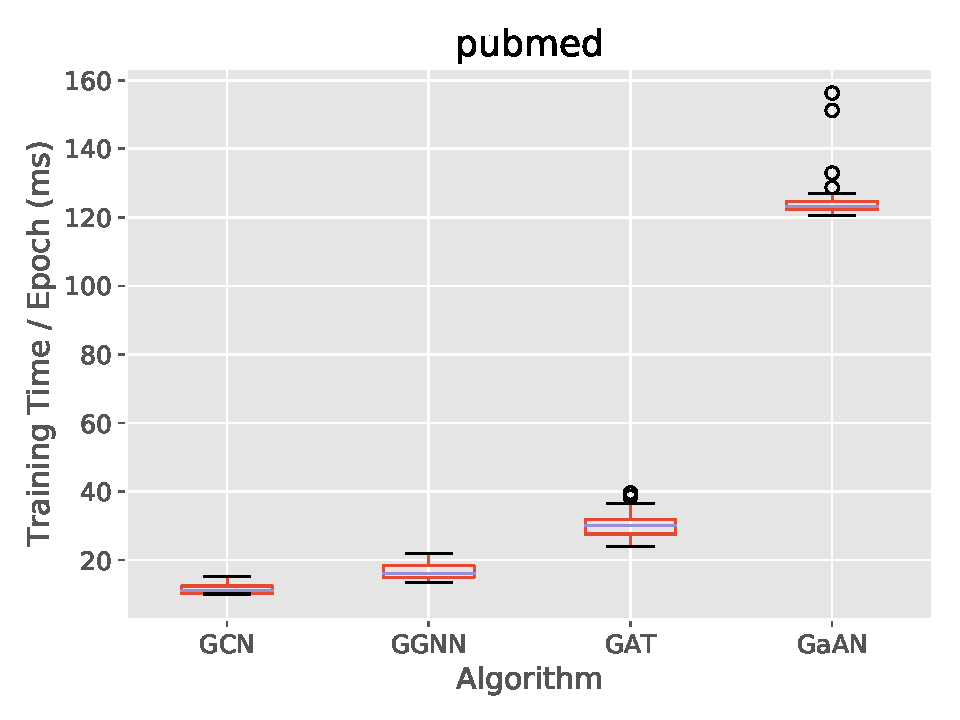
\includegraphics[height=4cm]{figs/experiments/exp_absolute_training_time_comparison_pubmed.pdf}}
    \subfloat[\texttt{aph}\label{fig:exp_absolute_training_time_amazon-photo}]{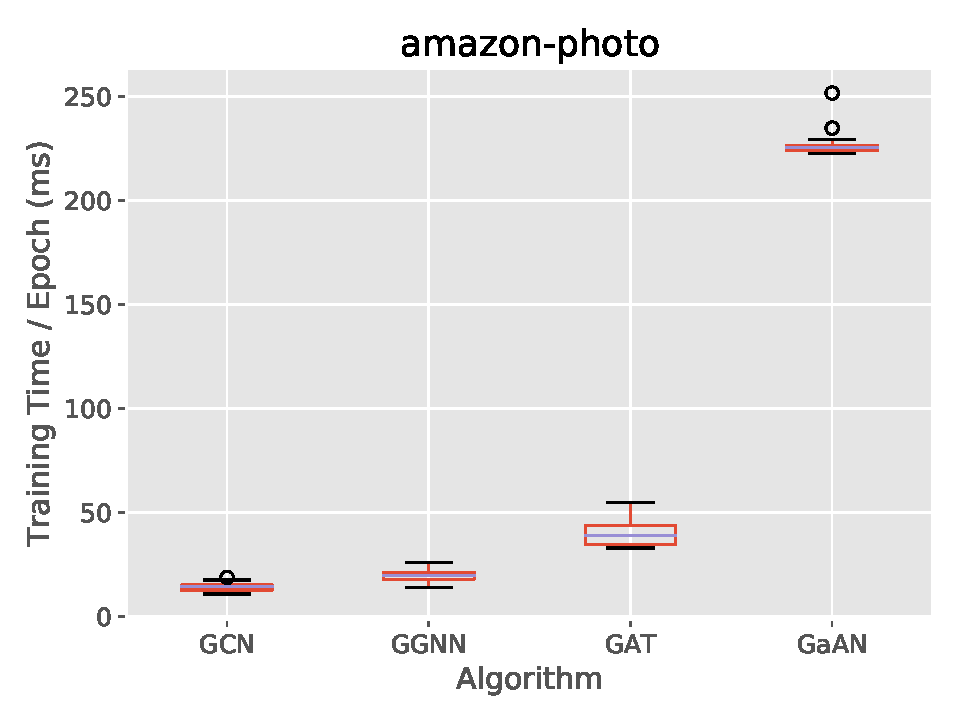
\includegraphics[height=4cm]{figs/experiments/exp_absolute_training_time_comparison_amazon-photo.pdf}}
    \subfloat[\texttt{cph}\label{fig:exp_absolute_training_time_coauthor-physics}]{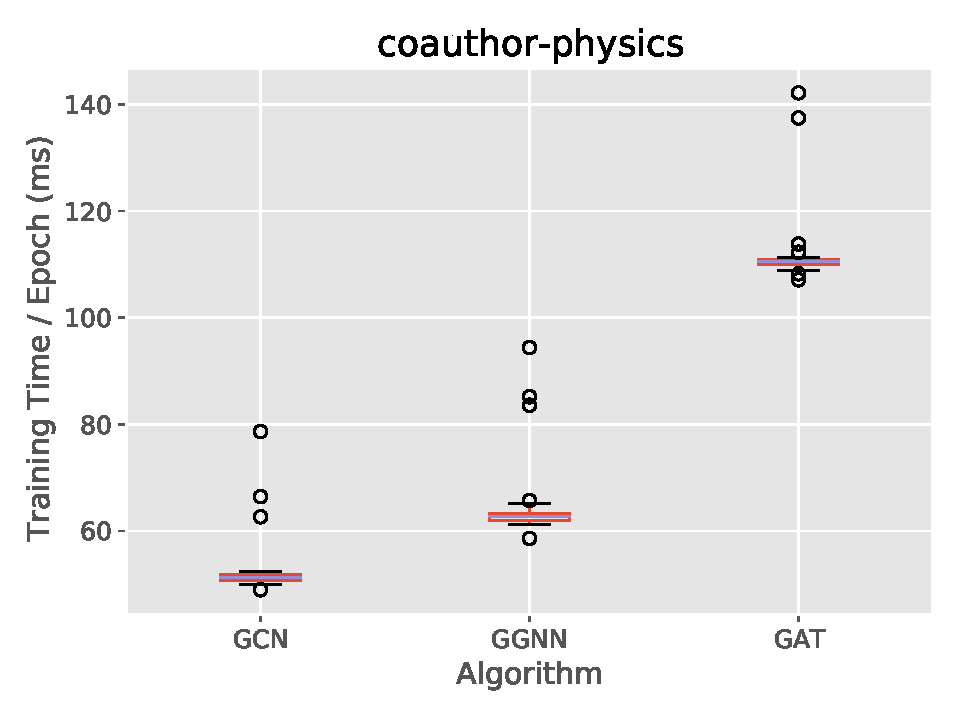
\includegraphics[height=4cm]{figs/experiments/exp_absolute_training_time_comparison_coauthor-physics.pdf}} \\
    \subfloat[\texttt{amc}\label{fig:exp_absolute_training_time_amazon-computers}]{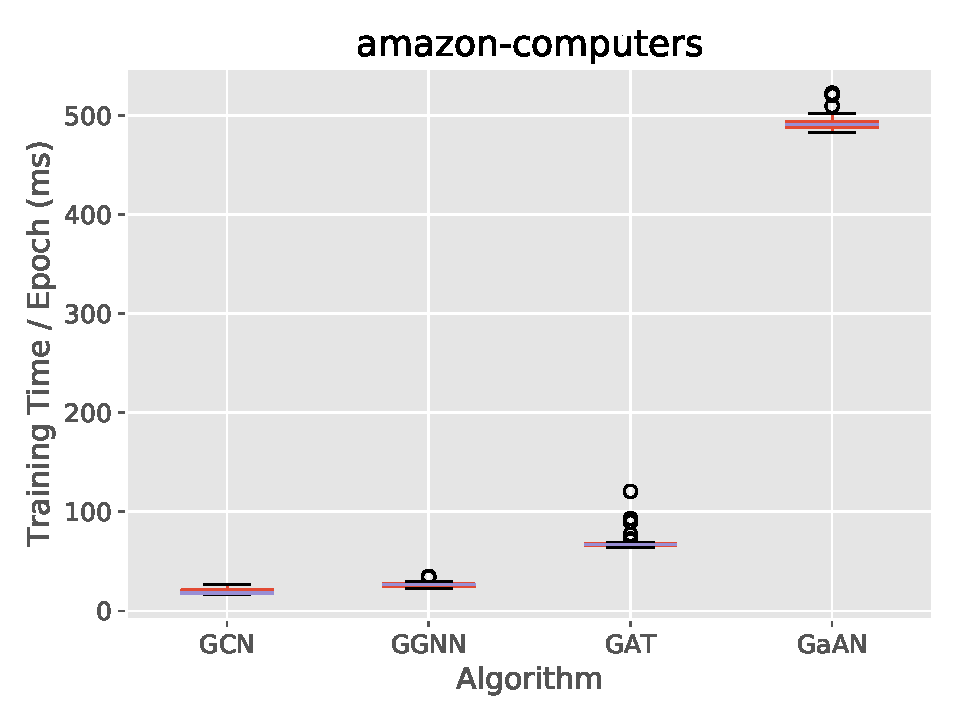
\includegraphics[height=4cm]{figs/experiments/exp_absolute_training_time_comparison_amazon-computers.pdf}}
    \subfloat[\texttt{fli}\label{fig:exp_absolute_training_time_flickr}]{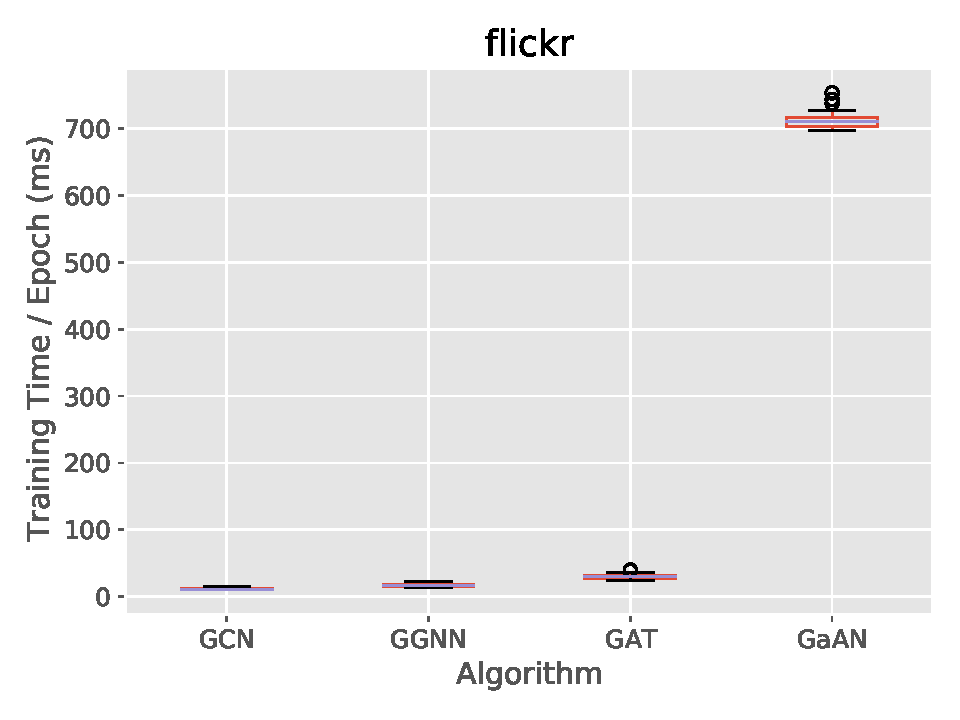
\includegraphics[height=4cm]{figs/experiments/exp_absolute_training_time_comparison_flickr.pdf}}
    \subfloat[\texttt{cam}\label{fig:exp_absolute_training_time_com-amazon}]{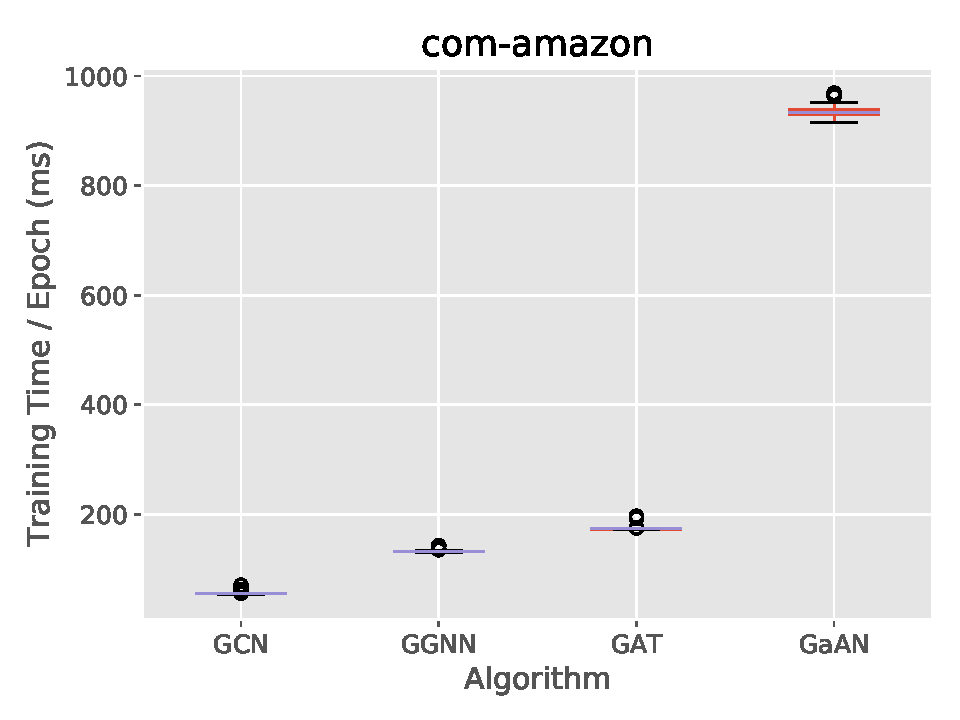
\includegraphics[height=4cm]{figs/experiments/exp_absolute_training_time_comparison_com-amazon.pdf}}
    \caption{Distribution of the wall-clock training time of 50 epoches on different datasets. GaAN crashed due to out of memory exception on the \texttt{cph} dataset.}
    \label{fig:exp_absolute_training_time}
\end{figure}

To further evaluate the effects of hyper-parameters, we measured the training time of each GNN with varying hyper-parameters in \figurename~\ref{fig:exp_hyperparameter_on_vertex_edge_phase_time}.

\begin{figure}
    \centering
    \subfloat[GCN\label{fig:exp_hyperparameter_on_vertex_edge_phase_time_gcn}]{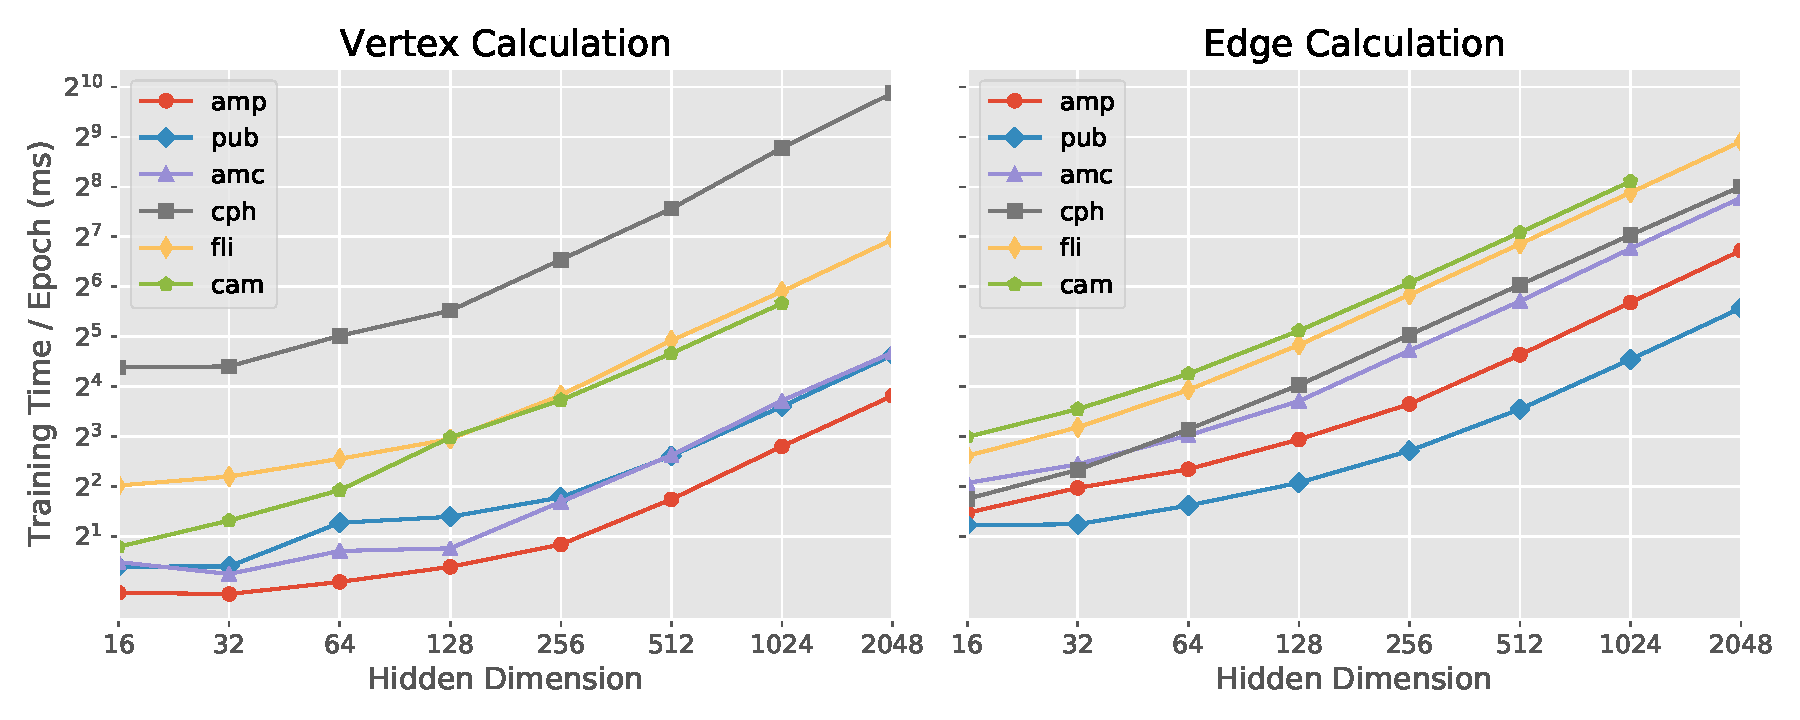
\includegraphics[height=3cm]{figs/experiments/exp_hyperparameter_on_vertex_edge_phase_time_gcn.pdf}}
    %
    \subfloat[GGNN\label{fig:exp_hyperparameter_on_vertex_edge_phase_time_ggnn}]{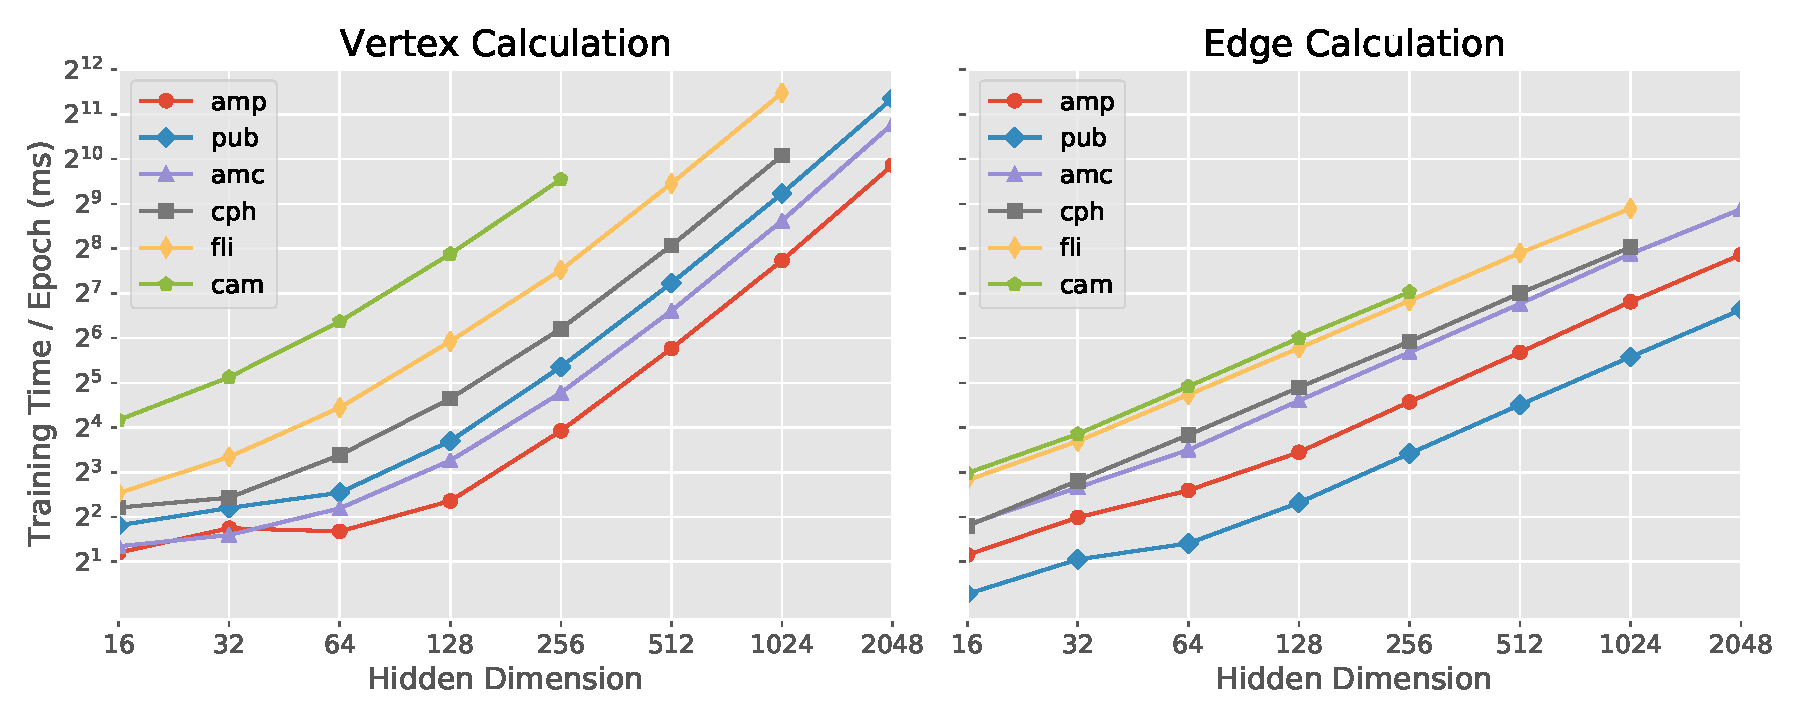
\includegraphics[height=3cm]{figs/experiments/exp_hyperparameter_on_vertex_edge_phase_time_ggnn.pdf}}
    \\
    \subfloat[GAT\label{fig:exp_hyperparameter_on_vertex_edge_phase_time_gat}]{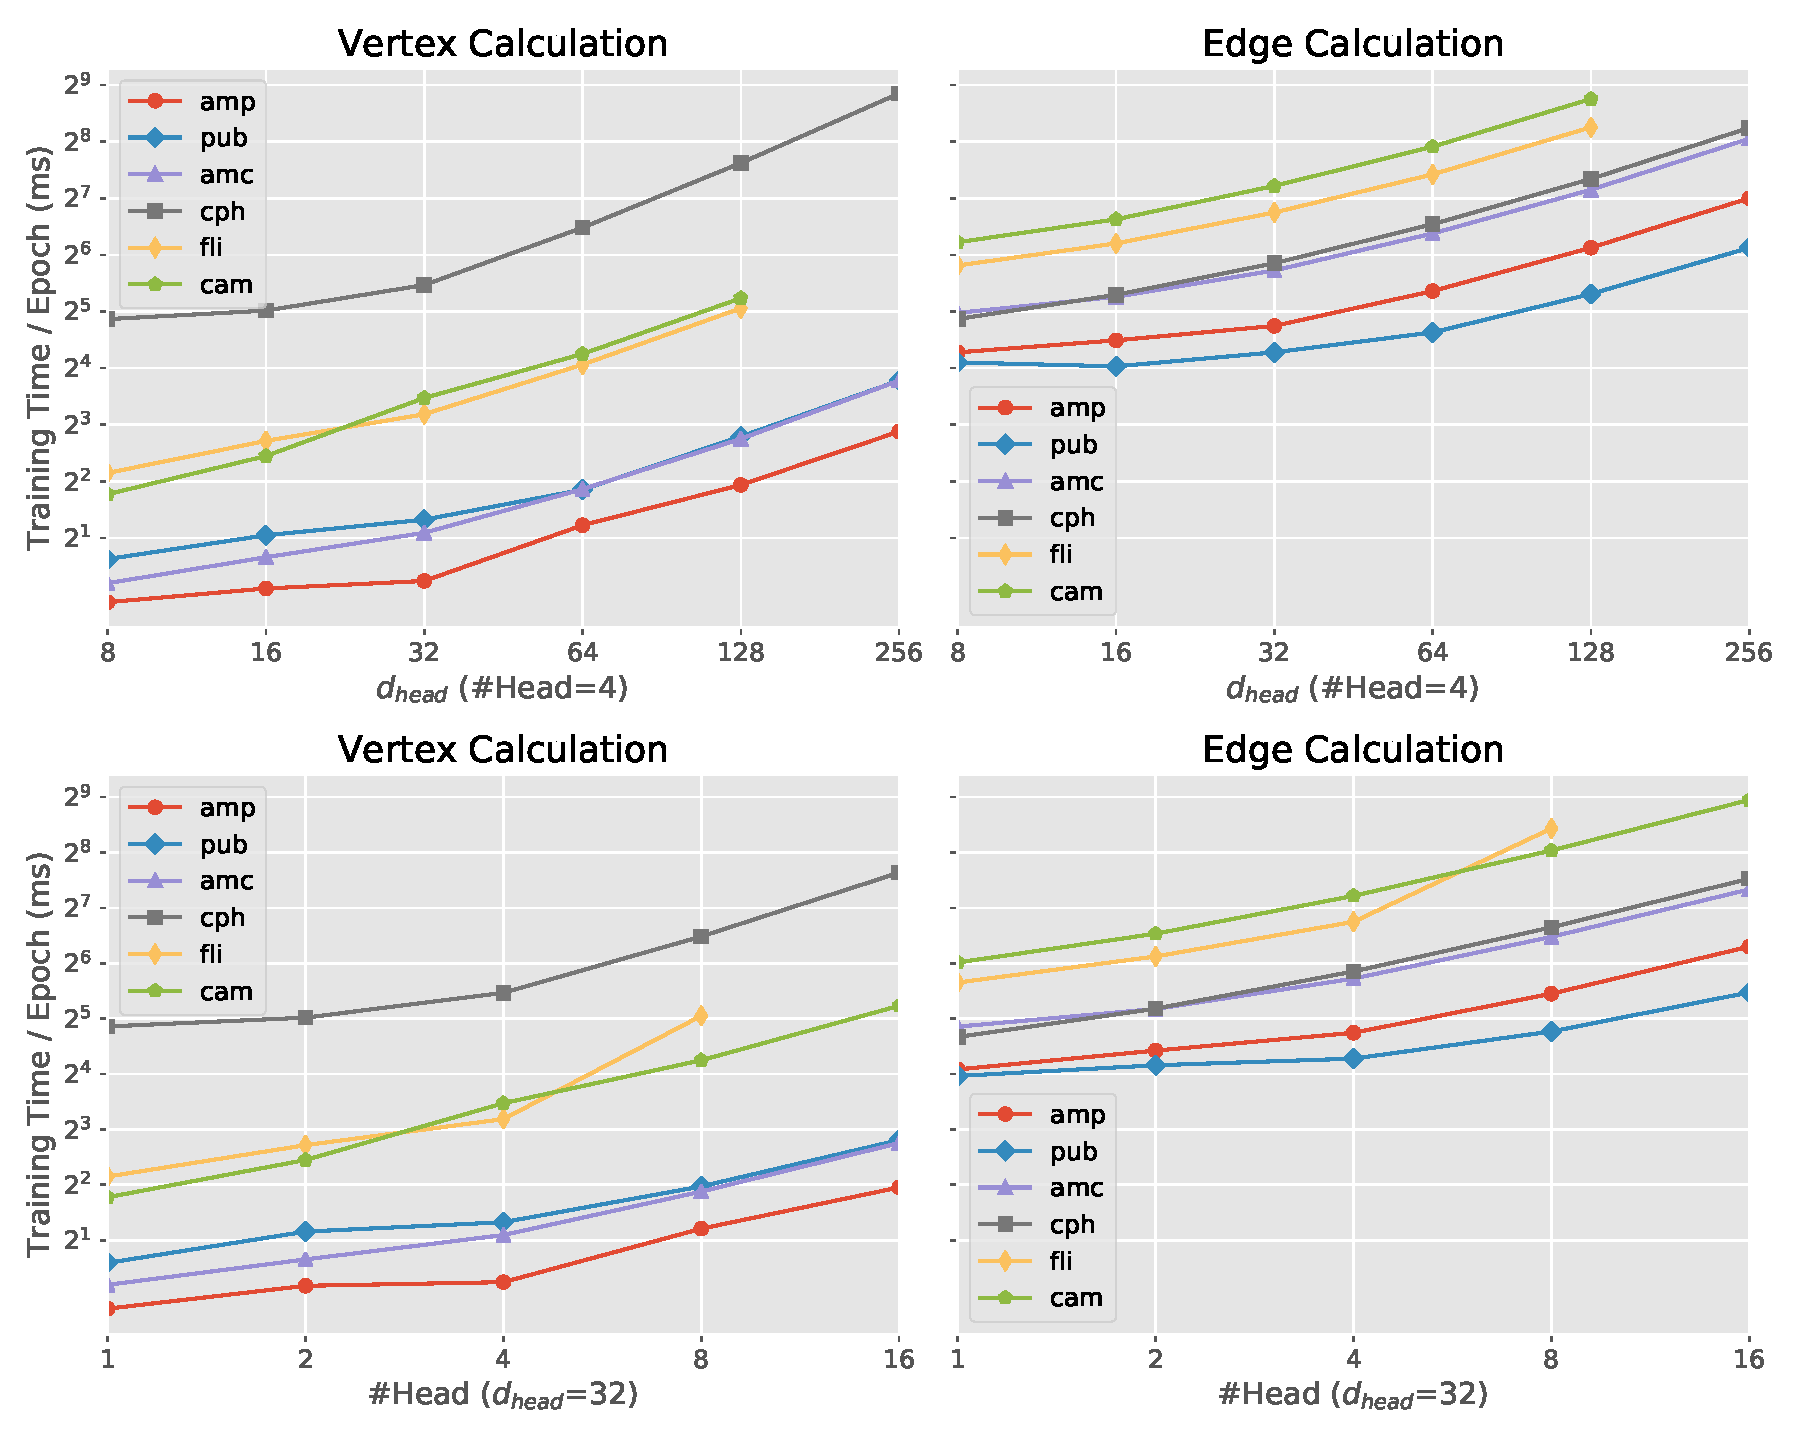
\includegraphics[height=6cm]{figs/experiments/exp_hyperparameter_on_vertex_edge_phase_time_gat.pdf}}
    \\
    \subfloat[GaAN\label{fig:exp_hyperparameter_on_vertex_edge_phase_time_gaan}]{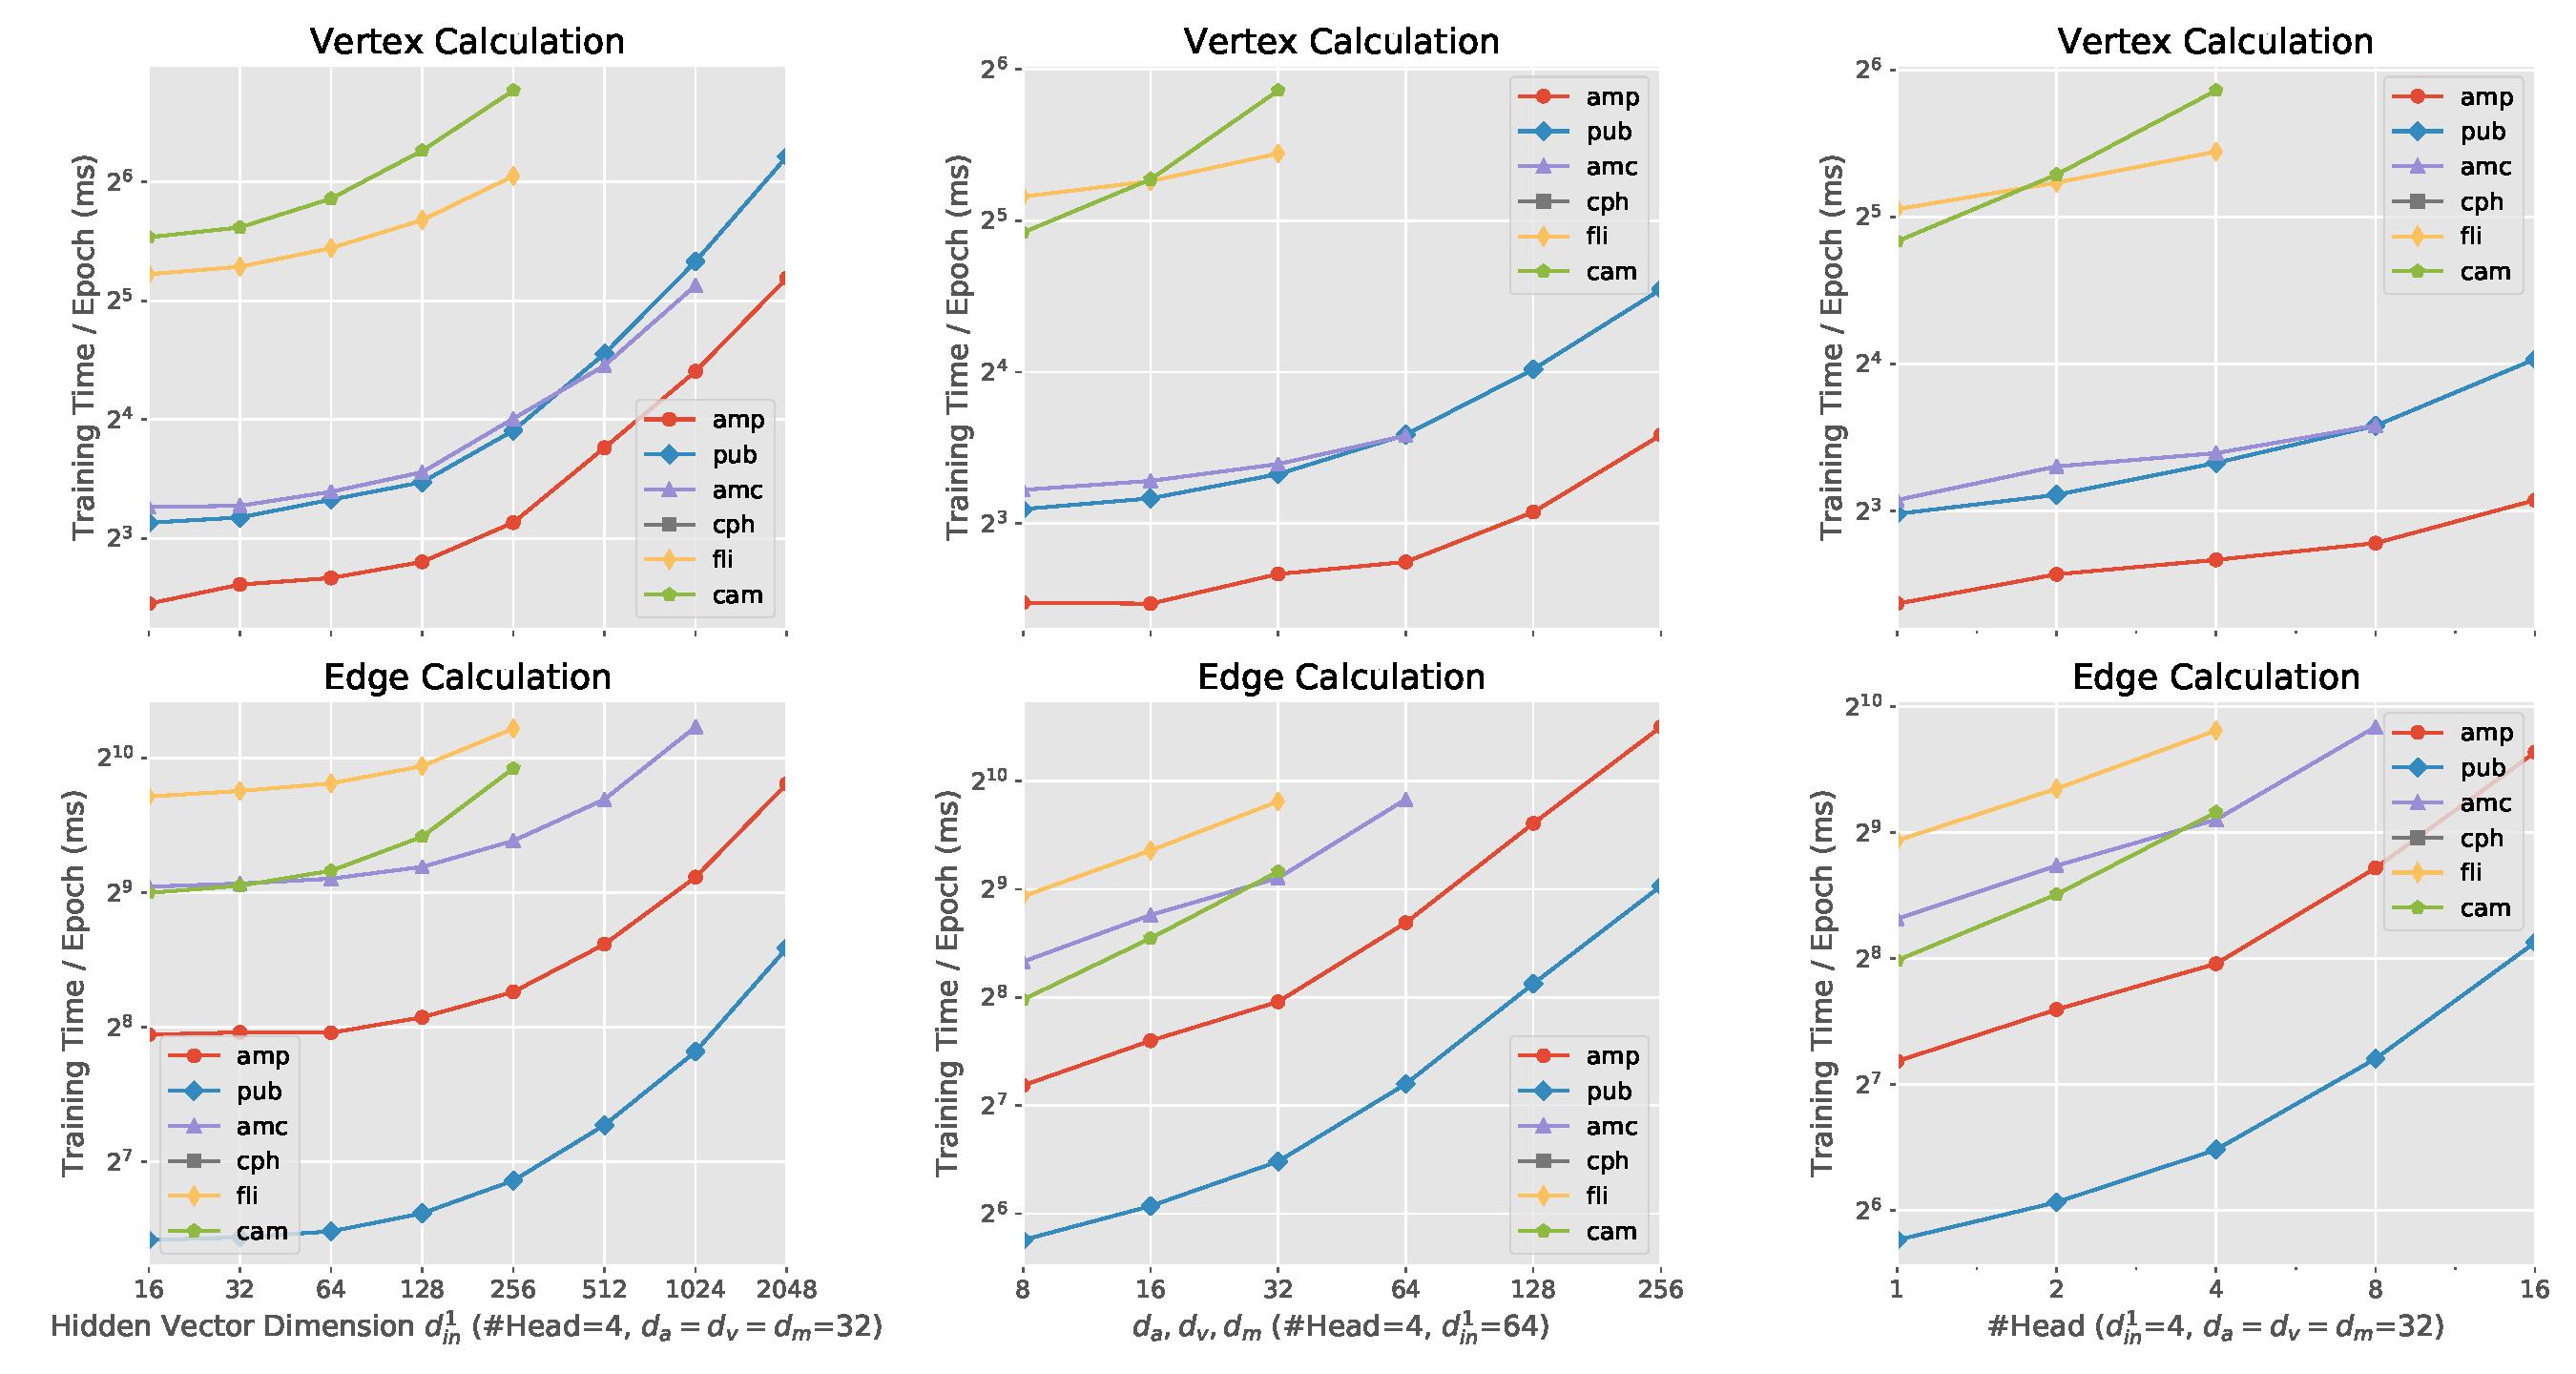
\includegraphics[height=6cm]{figs/experiments/exp_hyperparameter_on_vertex_edge_phase_time_gaan.pdf}}

    \caption{Effects of hyper-parameters on the vertex/edge calculation time.}
    \label{fig:exp_hyperparameter_on_vertex_edge_phase_time}
\end{figure}


For GCN and GGNN, the only modifiable hyper-parameter is the hidden dimension $dim(\boldsymbol{h}^1)$ with $dim(\boldsymbol{h}^1) = d^0_{out} = d^1_{in}$.
$dim(\boldsymbol{h}^0)$ and $dim(\boldsymbol{h}^2)$ is determined by the dataset with $dim(\boldsymbol{h}^0)=dim(\boldsymbol{x})$ and $dim(\boldsymbol{h}^2)=$\#Classes.
\figurename~\ref{fig:exp_hyperparameter_on_vertex_edge_phase_time_gcn} and \figurename~\ref{fig:exp_hyperparameter_on_vertex_edge_phase_time_ggnn} show that the training time of GCN and GGNN increased linearly under big $dim(\boldsymbol{h}^1)$, consistent with the time complexity analysis.

For GAT, we modified the number of heads $K$ and the dimension of each head $d_{head}$ in the GAT layer 0.
The dimenstion of the hidden feature vector was determined correspondingly as $d^0_{out} = d^1_{in} = dim(\boldsymbol{h}^1) = K h_{head}$.
\figurename~\ref{fig:exp_hyperparameter_on_vertex_edge_phase_time_gat} shows that the GAT training time increases linearly under big $d_{head}$ and $K$.

For GaAN, it is also based on the multi-head mechanism.
Its time complexity is affected by $d_{in}$, $d_v$, $d_a$ and the number of heads $K$.
\figurename~\ref{fig:exp_hyperparameter_on_vertex_edge_phase_time_gaan} demonstrates that the training time increased linearly with the hyper-parameters, except for $dim(\boldsymbol{h}^1)$.
As $dim(\boldsymbol{h}^1)$ increased, the training time increased first slightly and then linearly.
We could observe similar phenomena in GCN, GGNN and GAT with low hyper-parameters.
When the hyper-parameter was too low, the GNN training could not make use of the full computing power of the GPU.
When it became high enough, the training time increased linearly.

\begin{figure}
    \centering
    \subfloat[GCN]{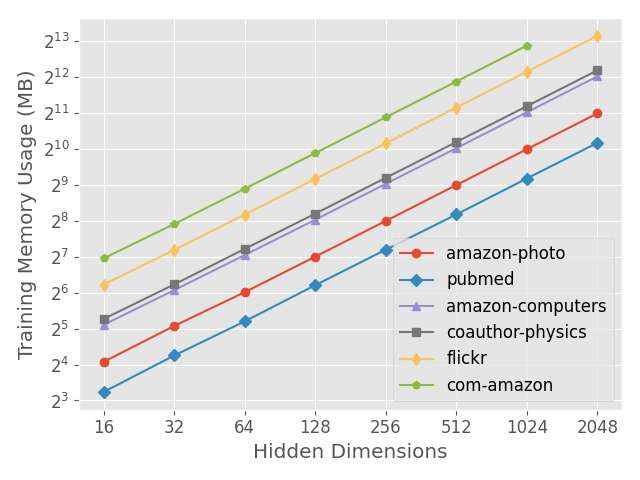
\includegraphics[height=3cm]{figs/experiments/exp_hyperparameter_on_memory_usage_gcn.png}}
    \subfloat[GGNN]{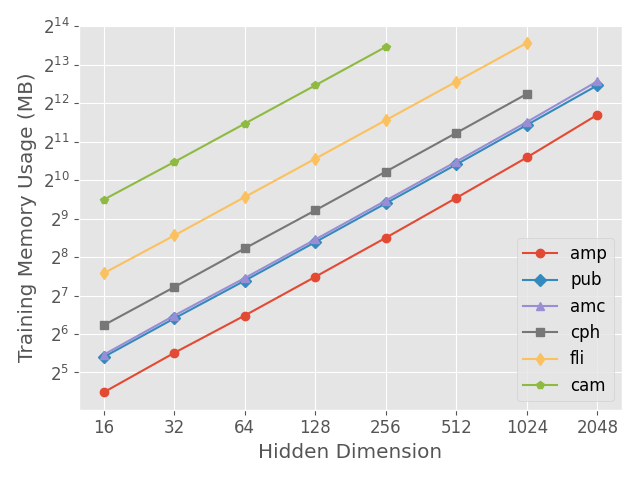
\includegraphics[height=3cm]{figs/experiments/exp_hyperparameter_on_memory_usage_ggnn.png}}\\
    \subfloat[GAT]{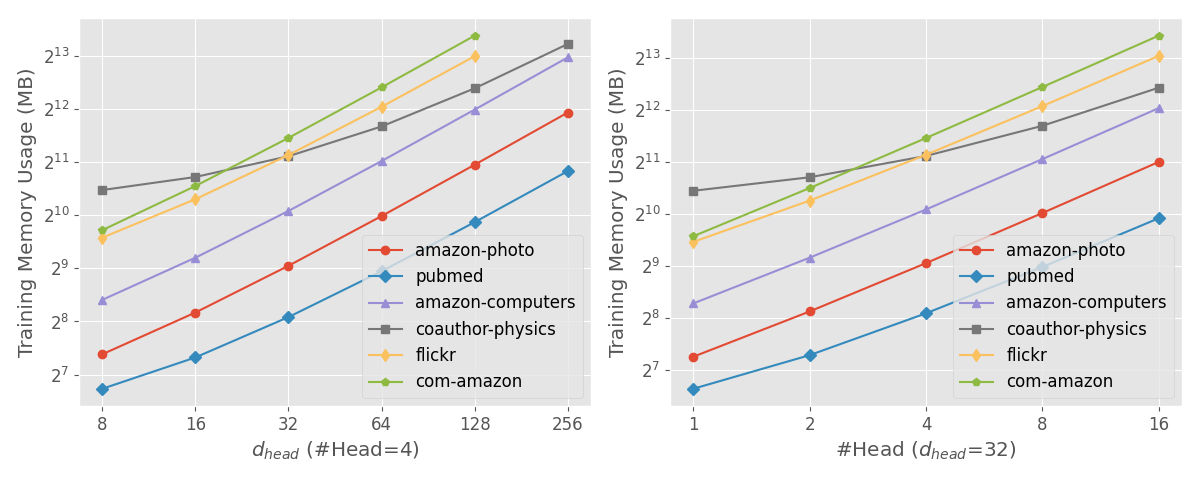
\includegraphics[height=3cm]{figs/experiments/exp_hyperparameter_on_memory_usage_gat.png}}\\
    \subfloat[GaAN]{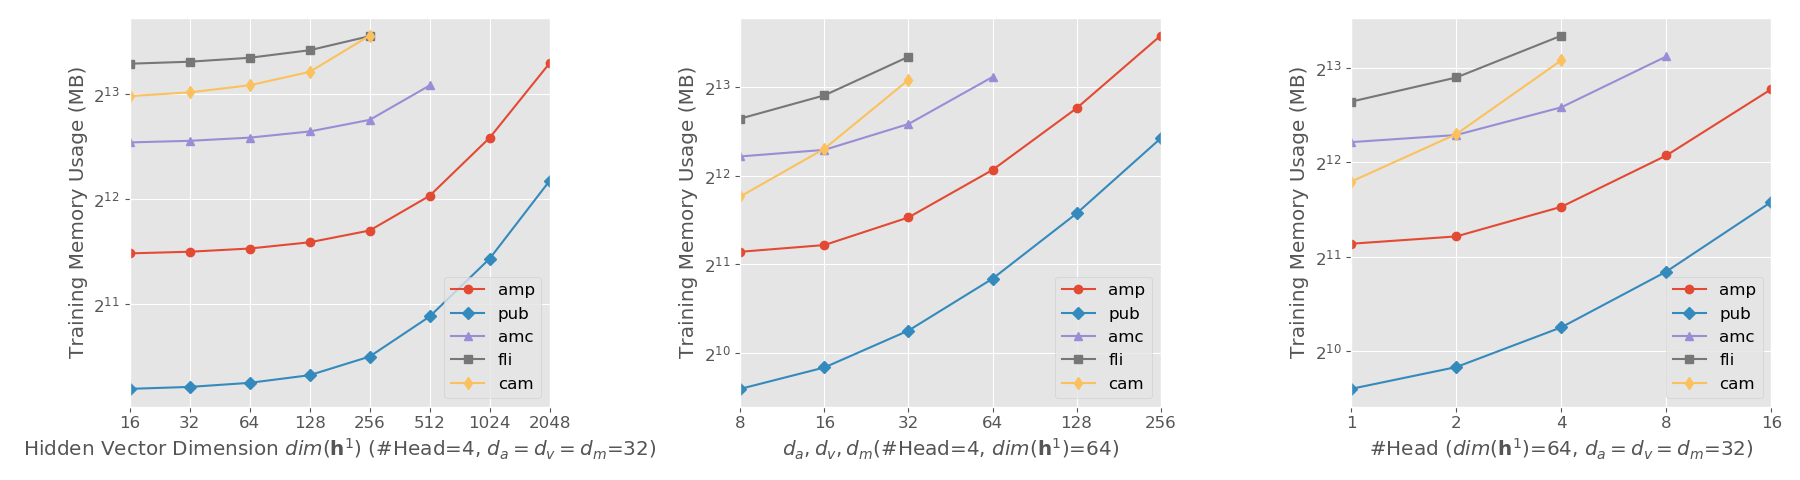
\includegraphics[height=3cm]{figs/experiments/exp_hyperparameter_on_memory_usage_gaan.png}}
    \caption{Effects of hyper-parameters on the peak GPU memory usage during the training, excluding the memory used by the dataset and the model parameters.}
    \label{fig:exp_hyperparameter_memory_usage}
\end{figure}

The experimental results support the time complexity analysis.
We further measured the effects of the hyper-parameters on the peak GPU memory usage in \figurename~\ref{fig:exp_hyperparameter_memory_usage}.
The memory usage also increased linearly as the hyper-parameters increased for all GNNs, except for GaAN on $dim(\boldsymbol{h}^1)$.
As the hidden feature vectors $\boldsymbol{h}^1$ consumed a small proportion of memory in GaAN, the growth in the memory usage was not noticable until $dim(\boldsymbol{h}^1)$ was large enough.

\paragraph{Summary}

The complexity analysis in \tablename~\ref{tab:gnn_overview_edge} and \tablename~\ref{tab:gnn_overview_vertex} is valid.
The hyper-parameters affect the training time and the memory usage of the GNN training \textbf{in a linear way}.
Algorithm enginners can use larger hyper-parameters to increase the expressive power of a GNN model without worrying the explosive growth in the training time and memory usage.

\subsection{Training Time Breakdown}
\label{sec:training_time_breakdown}

To find out which stage dominates the training time, we breakdown the training time and analyze the performance bottleneck level by level.

\subsubsection{Layer Level}

\begin{figure}
    \centering
    \subfloat[GCN]{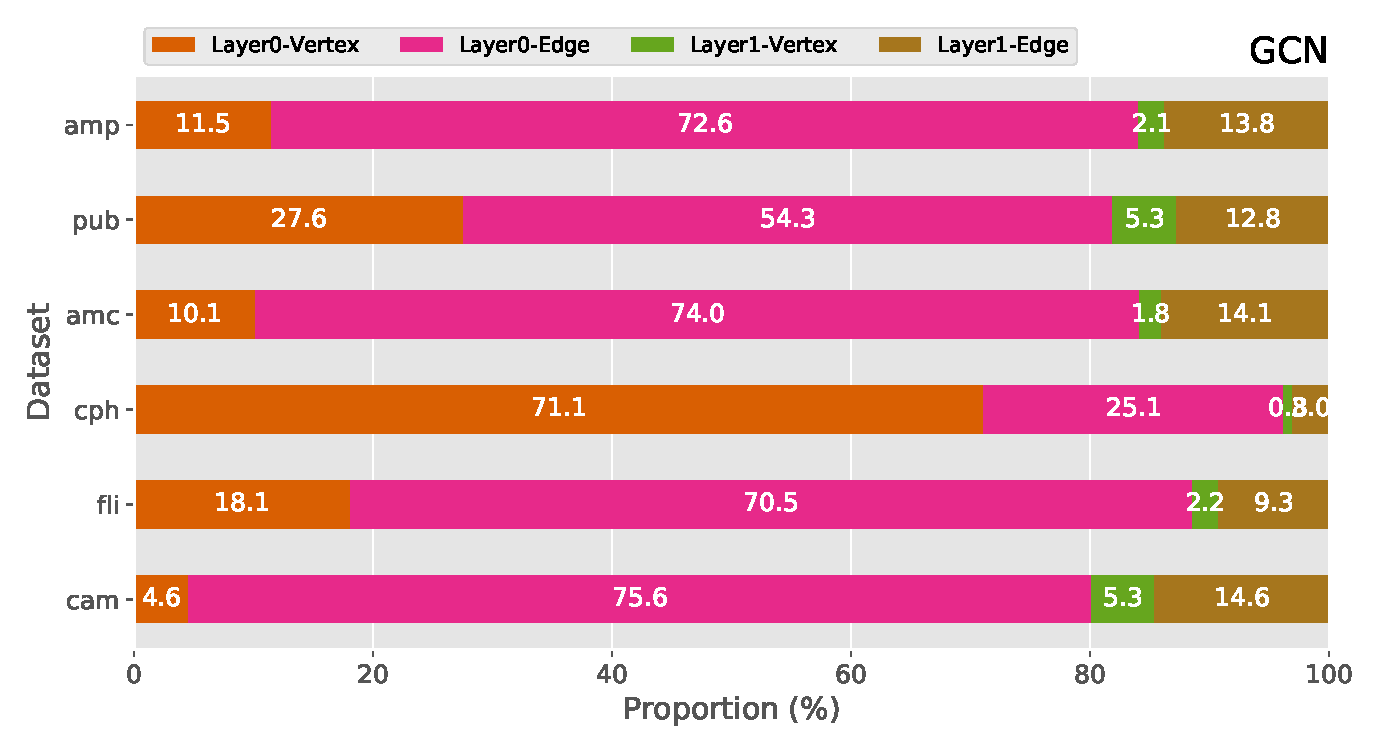
\includegraphics[height=4cm]{figs/experiments/exp_layer_time_proportion_gcn.pdf}}
    \subfloat[GGNN]{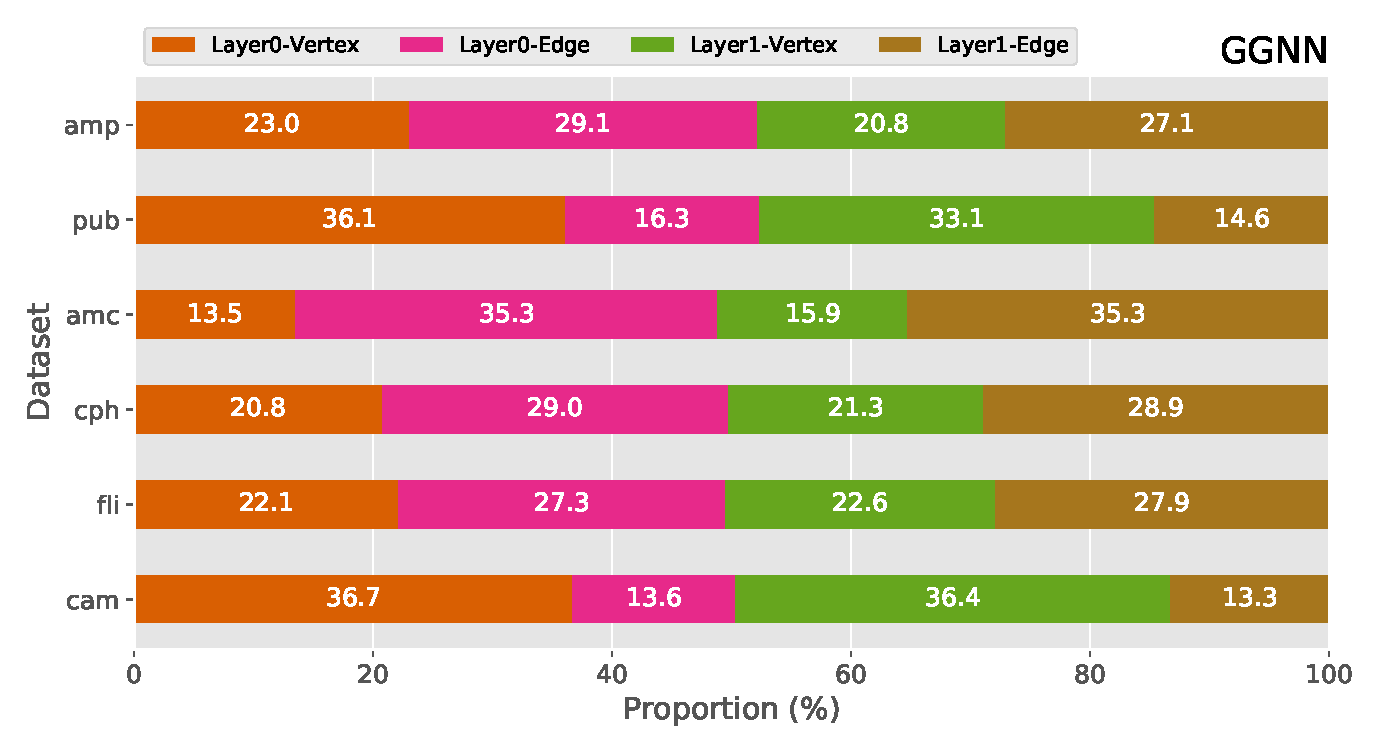
\includegraphics[height=4cm]{figs/experiments/exp_layer_time_proportion_ggnn.pdf}}\\
    \subfloat[GAT]{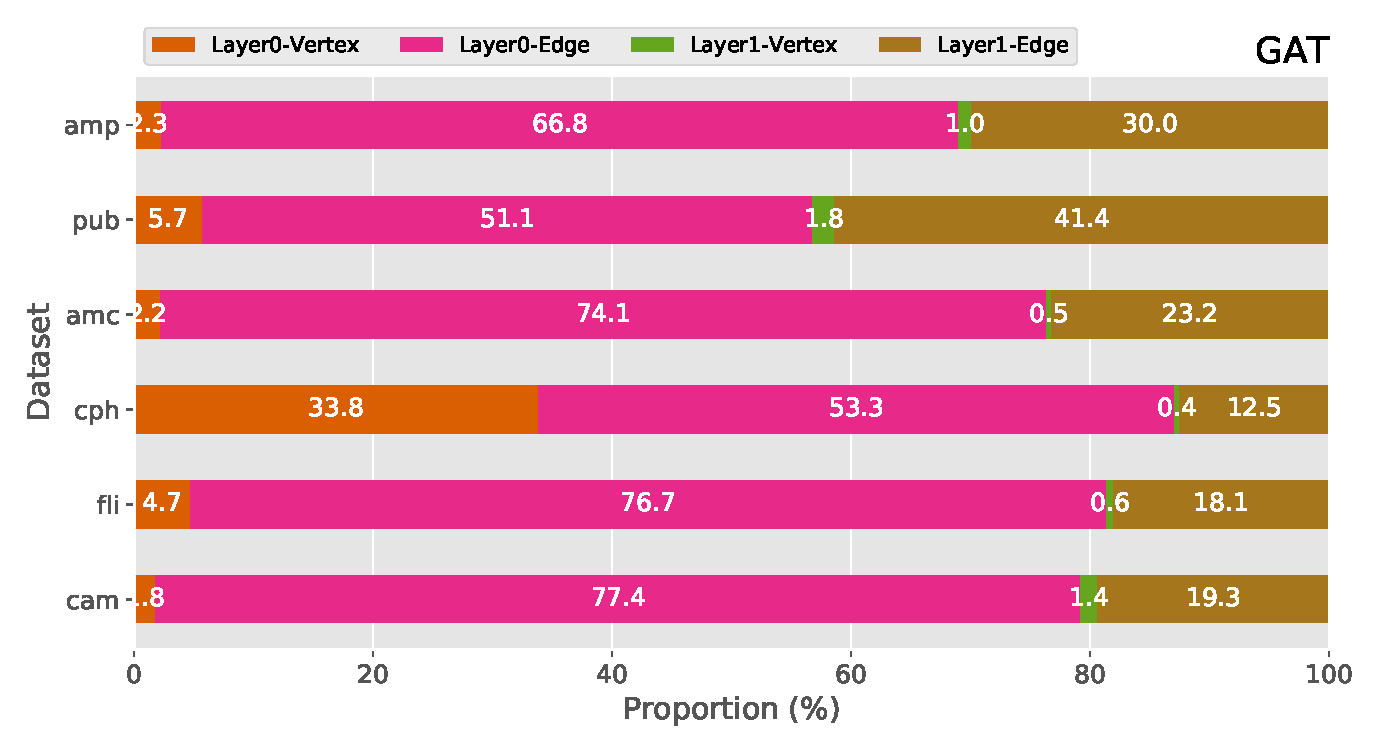
\includegraphics[height=4cm]{figs/experiments/exp_layer_time_proportion_gat.pdf}}
    \subfloat[GaAN]{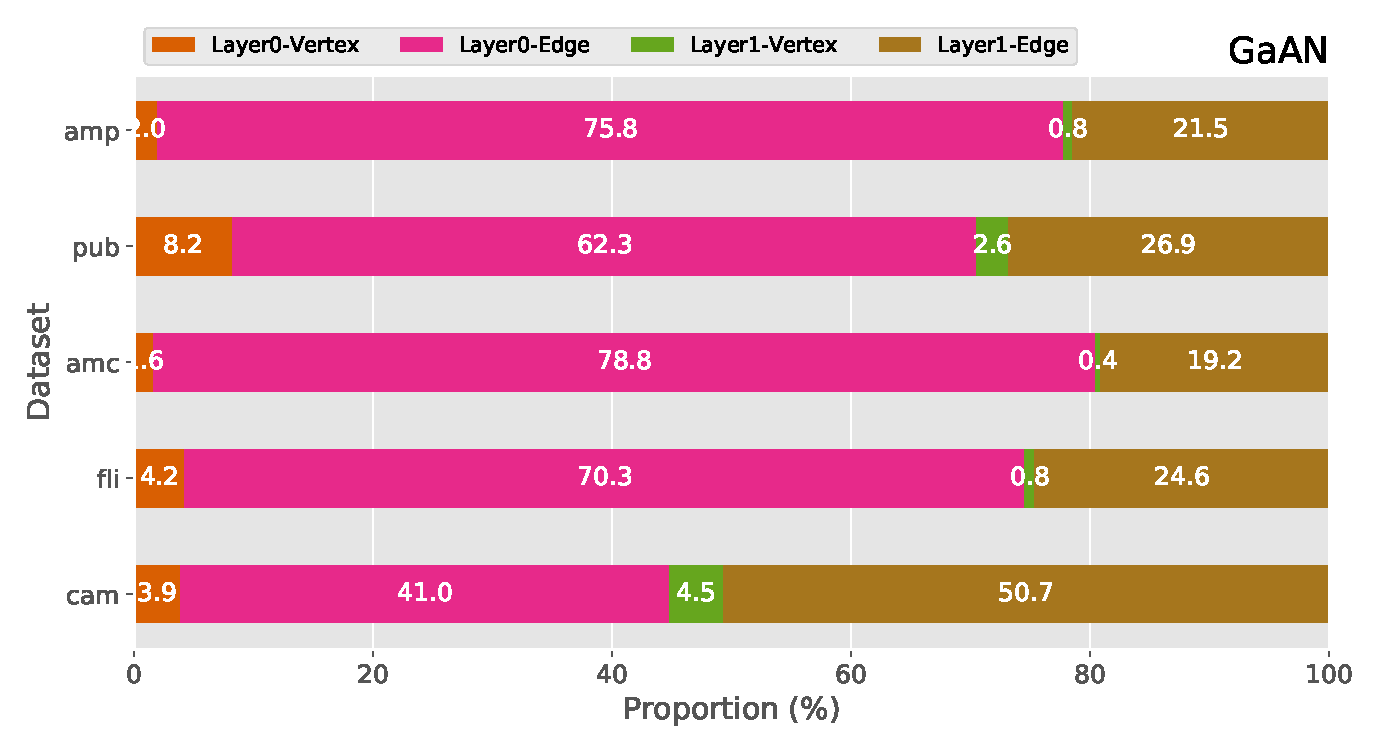
\includegraphics[height=4cm]{figs/experiments/exp_layer_time_proportion_gaan.pdf}}
    \caption{Training time breakdown on the layer level. The training time of each layer includes the time spent on the forward, backward and evaluation phases. Each layer is further decomposed into the vertex and the edge calculation stages.}
    \label{fig:exp_vertex_edge_cal_proportion}
\end{figure}

\figurename~\ref{fig:exp_vertex_edge_cal_proportion} decomposes the training time of a GNN on the layer level.
The training time of each layer is the summation of the time in the forward, backward and evaluation phases.
In GCN, GAT and GaAN, the time spent on the layer 0 was much larger than the layer 1.
In those GNNs, the dimensions of the input/output feature vectors in the layer 0 were much larger than the dimensions in the layer 1.
$d^0_{in}=dim(\boldsymbol{x})$, $d^0_{out}=d^1_{in}=64$ and $d^1_{out}=\#Class$ and $dim(\boldsymbol{x}) \gg \#Class$.
For GaAN, since it required the dimensions of the input/output feature vectors must be same, $d^0_{in}=d^0_{out}=d^1_{in}=d^1_{out}=64$ and the training time of both layers were close.

Each GNN layer can be further divided in the vertex and the edge calculation stages.
In \figurename~\ref{fig:exp_vertex_edge_cal_proportion}, GCN spent most of the training time on the edge calculation in most datasets.
A special case is \texttt{cph} dataset.
The dimension of the input feature vectors was very high in \texttt{cph}, making the vertex calculation stage of the GCN Layer 0 spend considerable time.
GGNN also spent the majority of its training time on the edge calculation.
But the high time complexity of its vertex update function $\gamma$ made the ratio of the vertex calculation in the total training time much higher than other GNNs.
%In \textit{pub} and cam dataset, the edge calculation cost and the vertex calculation cost are close for GGNN
%because the average degree of the two datasets is low (only 4.5 and 2.8).
For GAT and GaAN, due to their high edge calculation complexity, the edge calculation is the absolutely dominant stage.
In summary, \emph{the edge calculation is the most time-consuming stage in the GNN training}.

\begin{figure}
    \centering
    \subfloat[GCN]{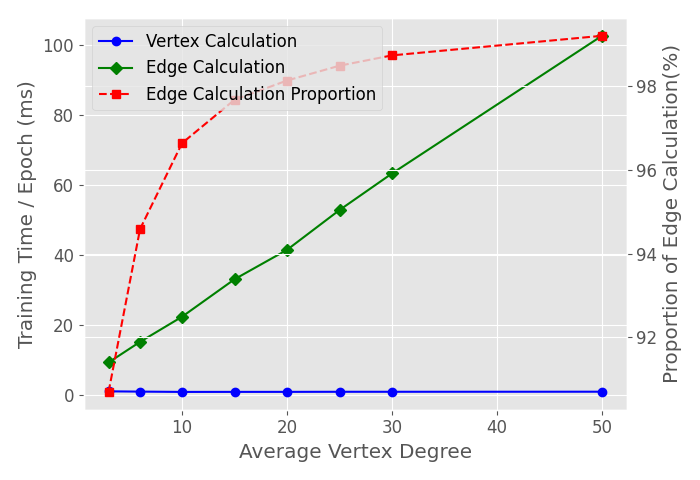
\includegraphics[height=4cm]{figs/experiments/exp_avg_degree_on_vertex_edge_cal_time_gcn.png}}
    \subfloat[GGNN]{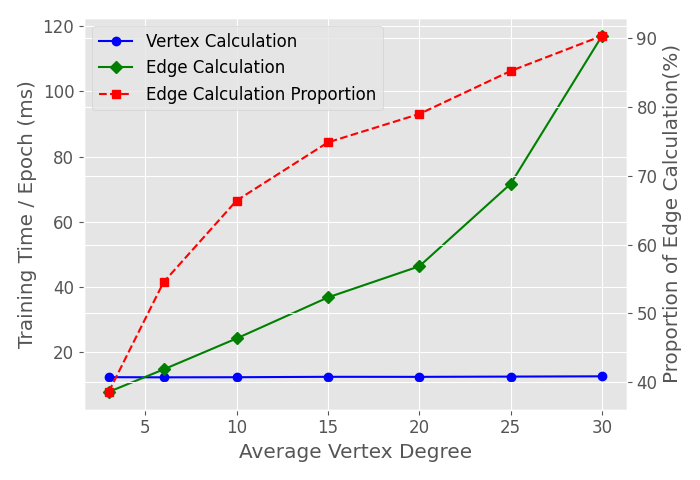
\includegraphics[height=4cm]{figs/experiments/exp_avg_degree_on_vertex_edge_cal_time_ggnn.png}}\\
    \subfloat[GAT]{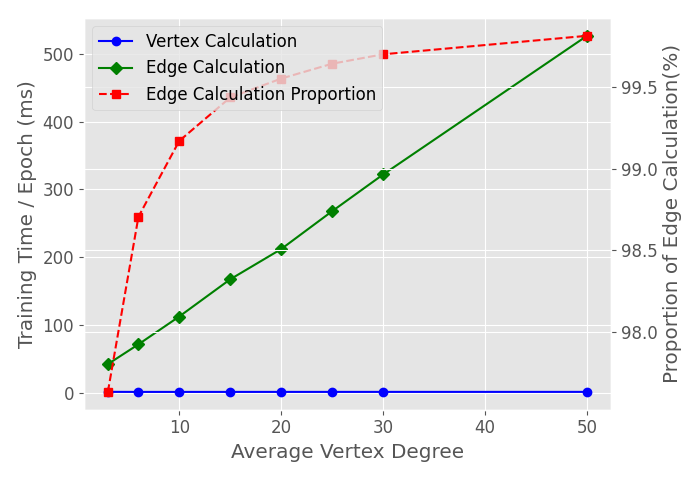
\includegraphics[height=4cm]{figs/experiments/exp_avg_degree_on_vertex_edge_cal_time_gat.png}}
    \subfloat[GaAN]{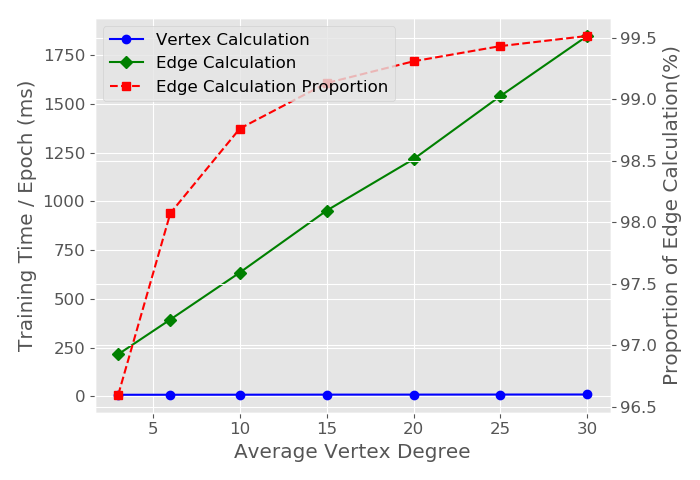
\includegraphics[height=4cm]{figs/experiments/exp_avg_degree_on_vertex_edge_cal_time_gaan.png}}
    \caption{Effects of the average degree on the time proportion of the vertex/edge calculation. Graphs were generated with the R-MAT generator by fixing the number of vertices as 50,000. }
    \label{fig:exp_avg_degree_on_vertex_edge_cal_time}
\end{figure}

The experimental results also indicate that the average degree of the dataset affects the time-consuming proportion of the vertex/edge calculation.
For GaAN, the time spent on the vertex calculation exceeded the edge calculation on the \texttt{pub} and \texttt{cam} datasets, because the avaerage degrees of the two datasets were low, making $|\mathcal{E}|$ and $|\mathcal{V}|$ much closer.
To evaluate the effects of the average degree, we used the R-MAT model to generate random graphs with 50k vertices and the average degrees ranging from 2 to 100.
\figurename~\ref{fig:exp_avg_degree_on_vertex_edge_cal_time} shows the training time of the four GNNs under different average degrees.
As the average degree increased, the training time of the edge calculation grew \emph{linearly}.
For GCN, GAT and GaAN, the edge calculation dominated the entire training time even under small average degrees.
Only for GGNN that had high vertex and low edge calculation complexities, the training time of the vertex calculation could exceed the edge calculation under low average degrees ($<5$).
Therefore, \emph{improving the efficiency of the edge calculation is the key to reduce the GNN training time}.

\subsubsection{Step Level in Edge Calculation}

\begin{figure}
    \centering
    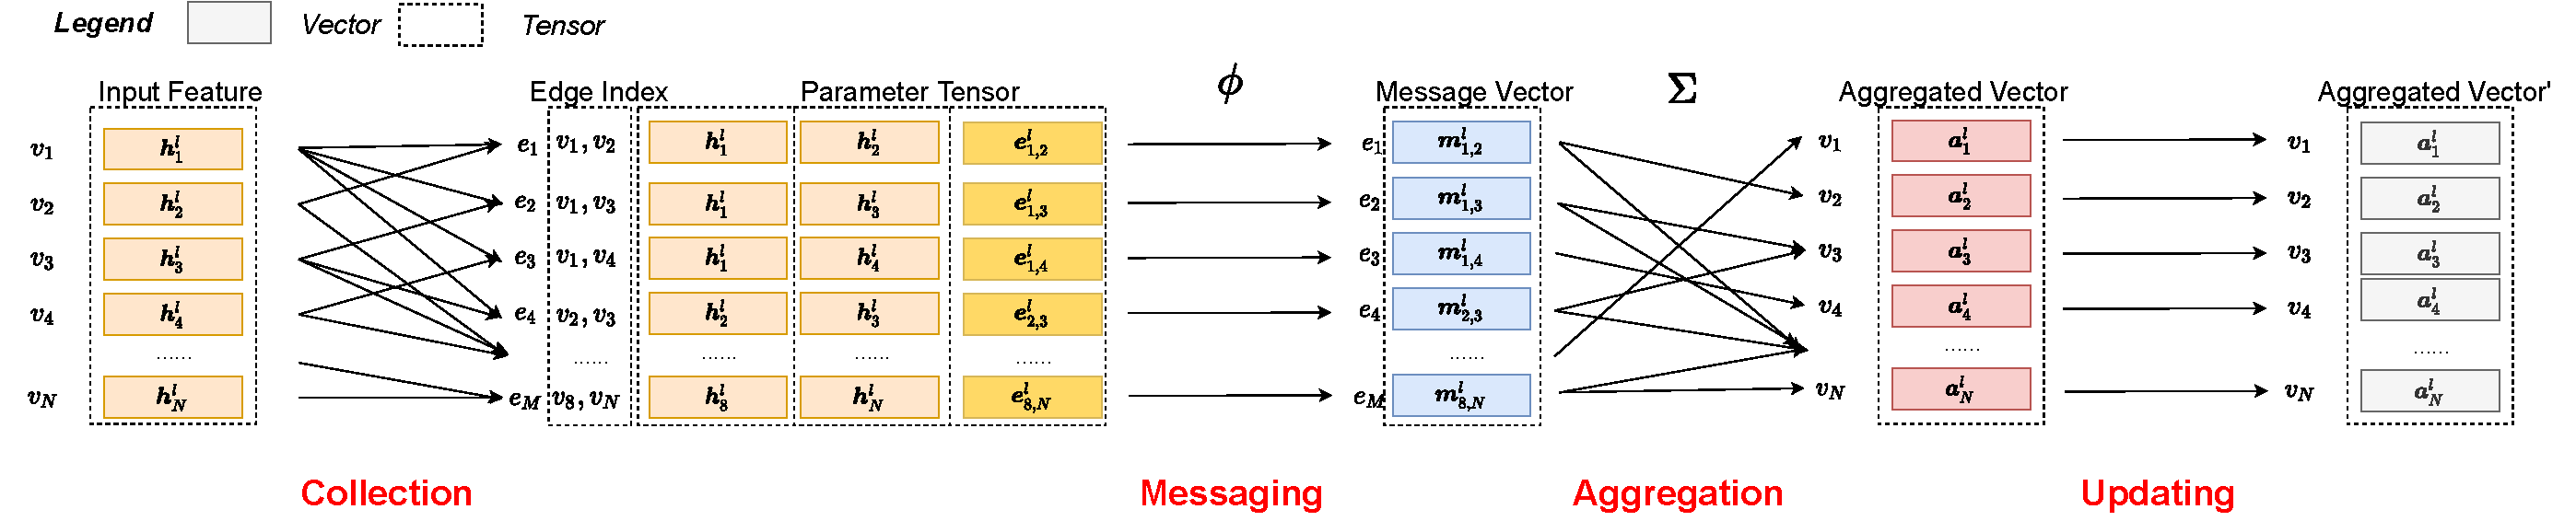
\includegraphics[width=1\columnwidth]{figs/illustration/steps_in_edge_calculation.pdf}
    \caption{Step decomposition of the edge calculation in the GNN layer $l$.}
    \label{fig:steps_in_edge_calculation}
\end{figure}

In the implementation of PyG, the edge calculation stage can be decomposed into four steps: collect, message, aggregate and update, as shown in \figurename~\ref{fig:steps_in_edge_calculation}.
The edge index is a matrix with $M$ rows and 2 columns that holds the edge set of the graph, where $M=|\mathcal{E}|$.
The two columns of the matrix store the source vertex and the target vertex of each edge, respectively.
The collect step copies the vertex feature vectors from the previous layer $\boldsymbol{h}_i^l$ to the ends of each edge 
in the edge index, to form the parameters $[\boldsymbol{h}^l_i, \boldsymbol{h}^l_{j}, \boldsymbol{e}^l_{i,j}]$ of the message function $\phi$.
This step only involves the data movement.
The message step calls the message function $\phi$ to get message vectors of all edges $\boldsymbol{m}_{i, j}^l$.
The aggregate step aggregates the message vectors with the same target vertex into a aggregated vector $\boldsymbol{s}^l_i$ with the aggregation operation $\Sigma$.
The update step is optinal.
It performs additional transformation on the aggregated vectors (for example, adding bias in GCN).
The aggregated vectors $\boldsymbol{s}^l_i$ (after the update step) will be fed into the vertex update function $\gamma$ as one of the input parameters.

\begin{figure}
    \centering
    \subfloat[GCN]{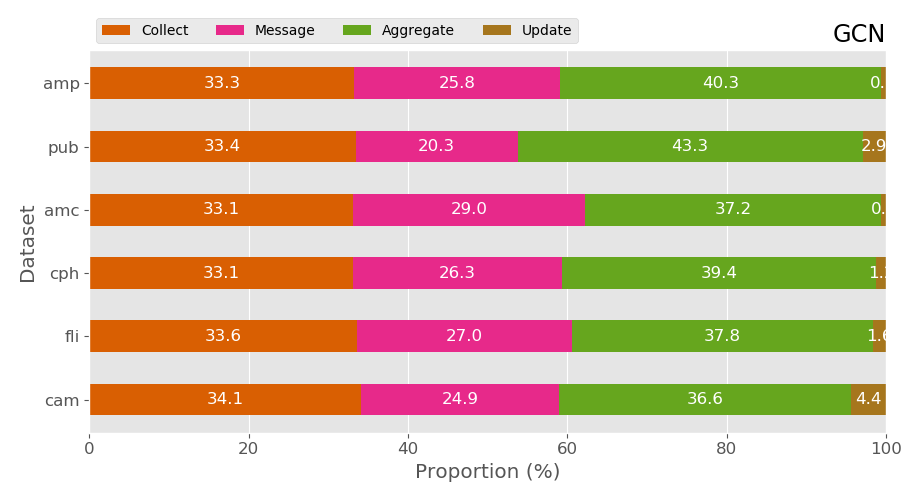
\includegraphics[height=4cm]{figs/experiments/exp_edge_calc_decomposition_gcn.png}}
    \subfloat[GGNN]{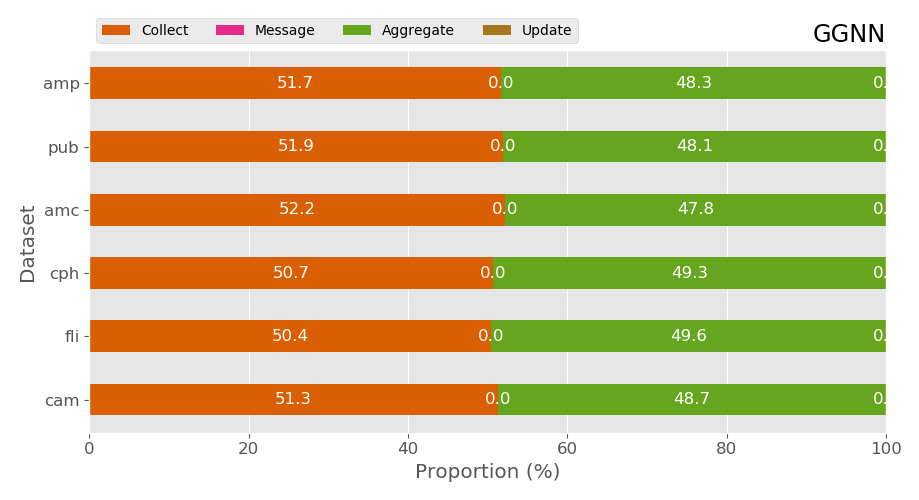
\includegraphics[height=4cm]{figs/experiments/exp_edge_calc_decomposition_ggnn.png}}\\
    \subfloat[GAT]{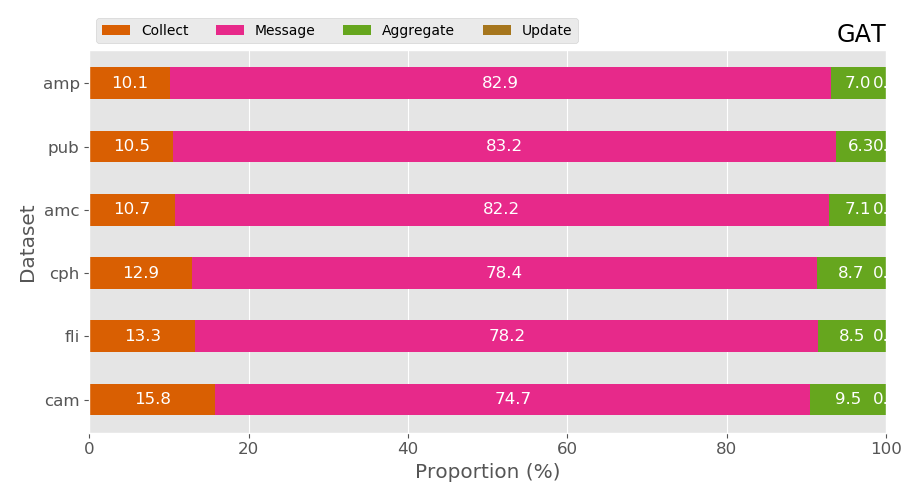
\includegraphics[height=4cm]{figs/experiments/exp_edge_calc_decomposition_gat.png}}
    \subfloat[GaAN]{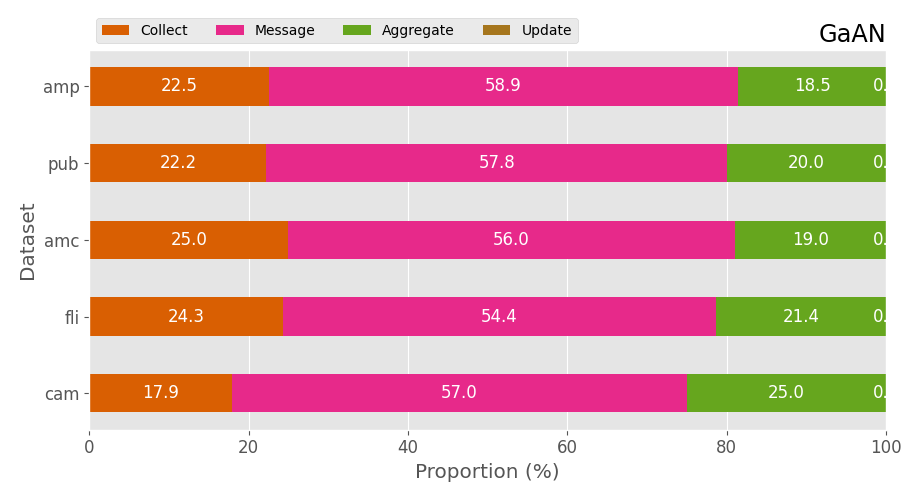
\includegraphics[height=4cm]{figs/experiments/exp_edge_calc_decomposition_gaan.png}}
    \caption{Training time breakdown of the edge calculation stage (including both GNN layers).}
    \label{fig:exp_edge_calc_decomposition}
\end{figure}

We decomposed the execution time of the edge calculation step in \figurename~\ref{fig:exp_edge_calc_decomposition}.
In each GNN, the proportion of the four steps were rather stable, rarely affected by datasets.
For GAT and GaAN with the high edge calculation complexity, the message step consumed most of the execution time.
For GCN and GGNN with the low complexity, the proportions of the steps were close.
Since the message function $\phi$ of GGNN used the pre-computed $\hat{\boldsymbol{h}}^l_i$ as the message vector directly in the implementation, the time spent on the message step of GGNN was negligible. 
Although the collect step did not conduct any computation and only involved data movement, it occupied noticeable execution time in all the GNNs.
The experiments show that \emph{the performance bottleneck on the step level depends on the complexity of the edge calculation}.
For GNNs with the high edge calculation complexity, the message function $\phi$ is the performance bottleneck.
Optimizing its implementation can significantly reduce the training time.
For the other GNNs, optimization should focus on reducing the costs of the collect and the aggregation steps.
Addtionally, improving the efficiency of the collect step can benefit all GNNs.

\subsubsection{Operator Level}

The functions $\phi$, $\Sigma$ and $\gamma$ in the vertex and edge calculation are made up of a series of basic operators implemented on GPU, like the matrix multiplication \texttt{mm}, the elementwise multiplication \texttt{mul} and the index-based selection \texttt{index\_select}.
\figurename~\ref{fig:exp_top_basic_ops} shows the five most time-consuming basic operators in each GNN, averaged over all the real-world graphs in \tablename~\ref{tab:dataset_overview}.

\begin{figure}
    \centering
    \subfloat[GCN]{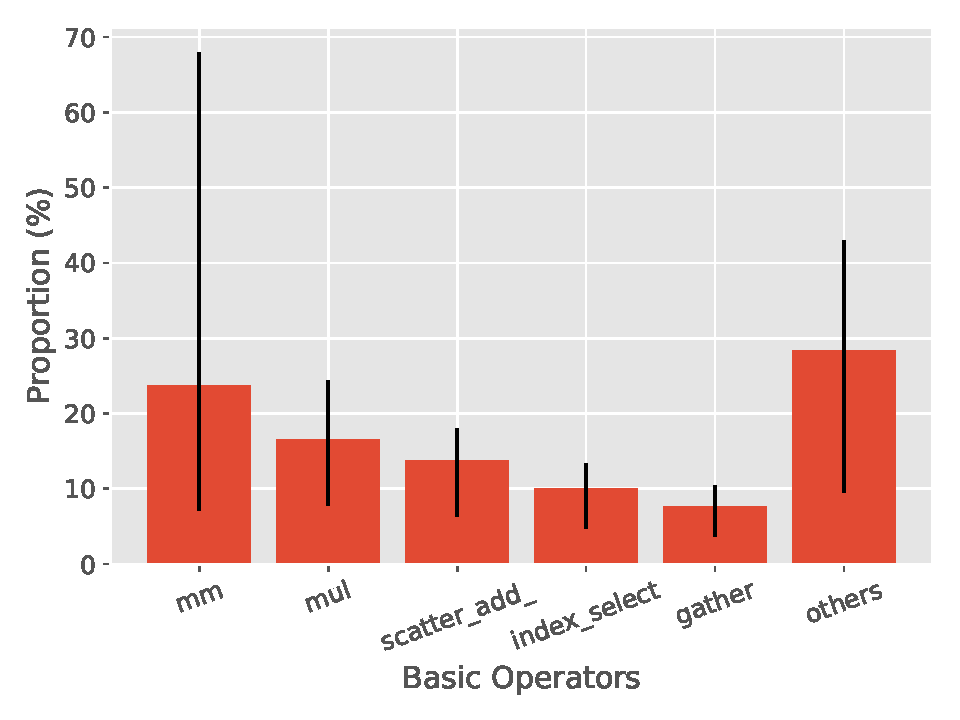
\includegraphics[height=4cm]{figs/experiments/exp_top_basic_ops_gcn.pdf}}
    \subfloat[GGNN]{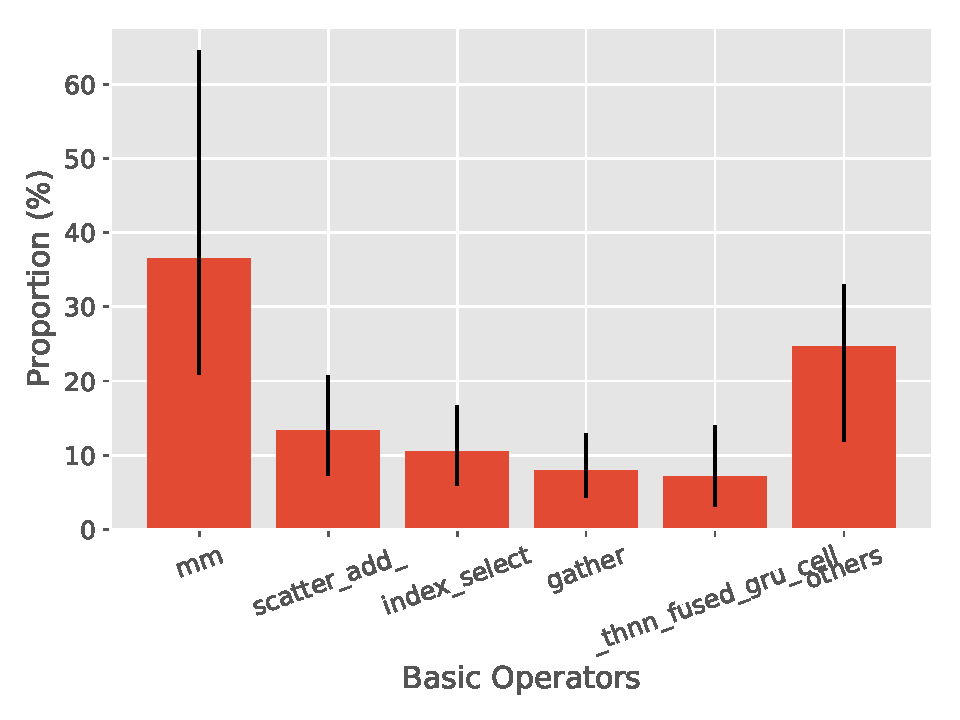
\includegraphics[height=4cm]{figs/experiments/exp_top_basic_ops_ggnn.pdf}}\\
    \subfloat[GAT]{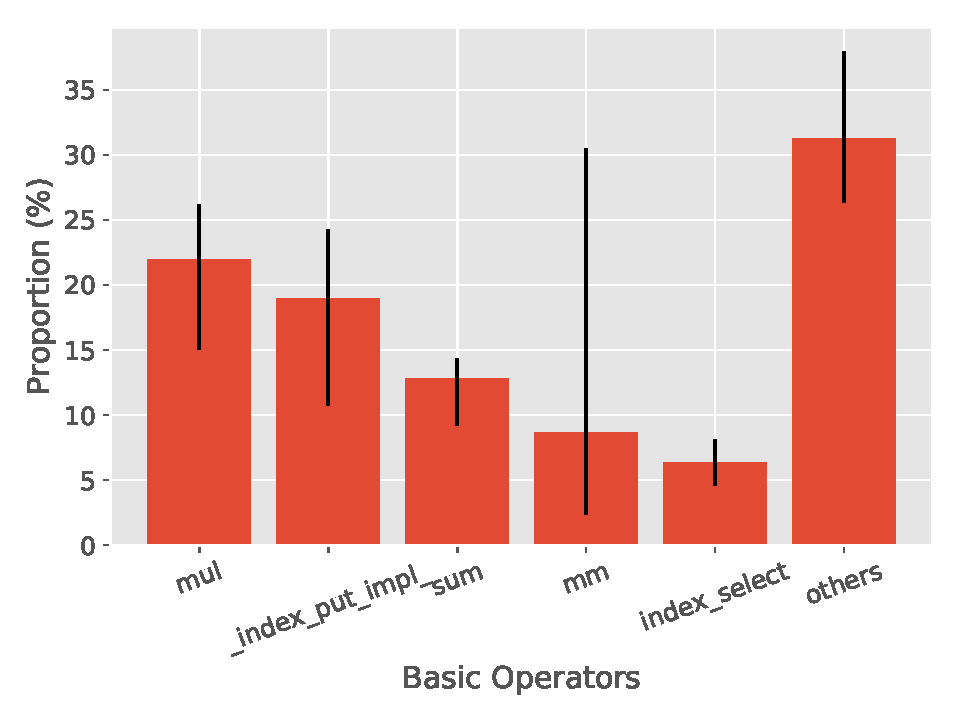
\includegraphics[height=4cm]{figs/experiments/exp_top_basic_ops_gat.pdf}}
    \subfloat[GaAN]{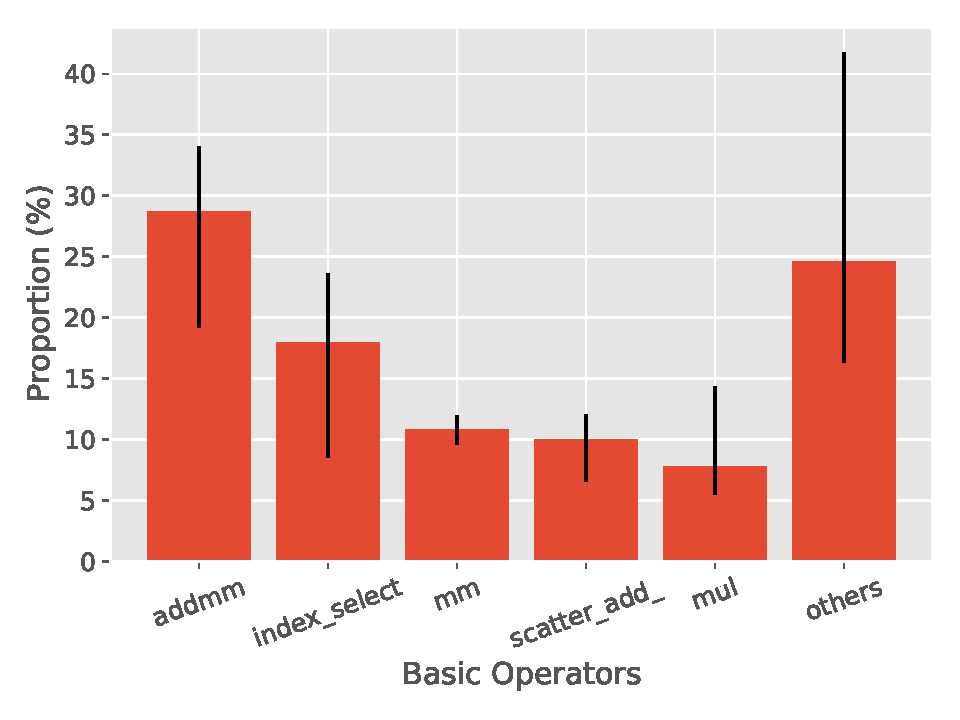
\includegraphics[height=4cm]{figs/experiments/exp_top_basic_ops_gaan.pdf}}
    \caption{Top 5 time-consuming basic operators of typical GNNs. The time proportion of each basic operator is averaged over all graphs with the error bar indicating the maximal and the minimal.}
    \label{fig:exp_top_basic_ops}
\end{figure}

\paragraph{GCN}
The most time-consuming basic operator was the matrix multiplication \texttt{mm} used in the vertex update function $\gamma$.
The elementwise multiplication \texttt{mul} used in the message function $\phi$ was also time-consuming.
The other three operators were used in the edge calculation: \texttt{scatter\_add\_} for the aggregation step in the forward phase, \texttt{gather} for the aggregation step in the backward phase, and \texttt{index\_select} for the collect step.
For GCN, the basic operators related to the edge calculation consumed the majority of the training time.

\paragraph{GGNN}
The top basic operator was \texttt{mm} used in the vertex calculation.
Due to the high time complexity in $\gamma$, the proportion of the \texttt{mm} operator were much higher than the other operators.
The \texttt{thnn\_fused\_gru\_cell} operator that was used in the backward phase of $\gamma$ was also noticeable.
The other three operators were used in the edge calculation.

\paragraph{GAT}
All the top basic operators except for \texttt{mm} were related to the edge calculation.
The \texttt{mm} operator was used in the vertex update function $\gamma$.

\paragraph{GaAN}
The top basic operator was \texttt{mm}.
It was used in both the vertex and the edge calculation, where the edge calculation is dominant.
The scalar multiplication \texttt{mul} and the concatenation \texttt{cat} operators were used in the message function $\phi$.

In general, the most time-consuming operator in GNN calculation is still the matrix multiplication \texttt{mm} and the elementwise multiplication \texttt{mul}, \emph{making GNN training suitable for GPU}.
Although the aggregate step in the edge calculation is relatively simple (like sum and mean), the related operators \texttt{scatter\_add} and \texttt{gather} still consumed a certain amount of the time.
They have to synchronize between hardware threads to avoid updating the same aggregated vector at the same time and they conducted non-regular memory access with the access pattern determined by the edge set dynamically.
For GPU, they were less efficient than \texttt{mm}.
The index-based selection \texttt{index\_select} operator from the collection step consumed around 10\% of time in all GNNs.
Though GPUs have high on-chip memory bandwidth, improving the efficiency of \texttt{scatter\_add}/\texttt{gather}/\texttt{index\_select} (like overlapping them with $\phi$) can benifit the training of all kinds of GNNs.

\paragraph{Summary}
The GNN training is suitable for GPU.
The \textbf{edge calculation is the main performance bottleneck}, except for training GNNs with high vertex calculation complexity on low-average-degree graphs.
The performance bottleneck in the edge calculation depends on the time complexity of the message function $\phi$.
\begin{itemize}
    \item If the time complexity of $\phi$ is \textbf{high}, the \textbf{efficiency of $\phi$} limits the performance. Reducing its computation cost (via optimizing its implementation or modifying the algorithm) can significantly reduce the training time.
    \item If the time complexity of $\phi$ is \textbf{low}, the \textbf{collect step} and the \textbf{aggregation step} limit the performance. The collect step involves lots of data movement. The aggregation step suffers from the data synchronization and non-regular data access. Optimizing their implementations can significantly reduce the training time.
\end{itemize}

\subsection{Memory Usage Analysis}

At present, all data (including datasets and intermediate calculation results) of PyG in the process of training GNN with GPU
are stored in GPU memory. Compared with the main memory of the system, the memory capacity on GPU is very limited.
\textbf{GPU memory capacity is limited to Determinants of the size of the training dataset}.
GaAN was unable to complete the training due to memory overflow during the training of the `\textit{cph}` dataset.

\begin{figure}
    \centering
    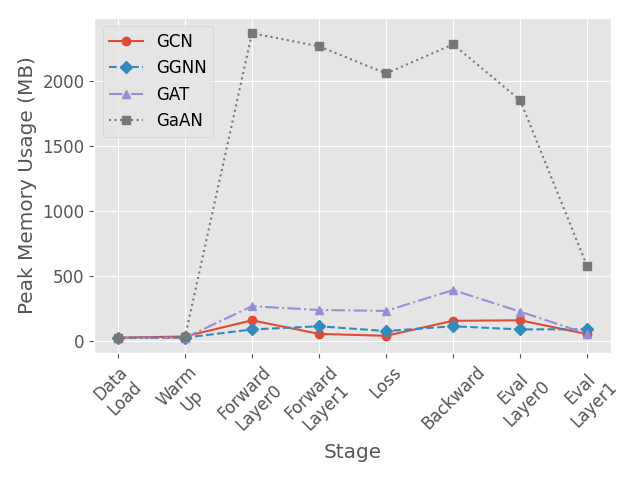
\includegraphics[width=0.7\columnwidth]{figs/experiments/exp_memory_usage_stage_amp.png}
    \caption{Maximum memory usage in each stage. Data Load refers to memory usage after data is loaded. dataset: amp. Other datasets are similar}
    \label{fig:exp_memory_usage_stage_amp}
\end{figure}

\figurename~\ref{fig:exp_memory_usage_stage_amp} shows the peak memory usage of each stage when each GNN is trained on the cam dataset, the situation is similar on other datasets.
\textbf{The memory usage in GNN training is forward The peak in the phase and the backward phase},
because a large number of temporary calculation results will be generated in the forward phase,
and the key intermediate calculation results will be cached.
The cached intermediate results will be used in the gradient calculation of the backward phase.
\figurename~\ref{fig:ggnn_vertex_func_computation_graph} shows the calculation graph of GGNN's vertex calculation function $\gamma$.
It can be seen that a large number of operators are involved in GGNN vertex calculation and a large number of intermediate calculation results are generated.The key calculation results will also be cached,
which is exacerbated Memory usage. Most of the peak memory usage in the loss phase comes from the intermediate calculation results of the cache.
With the end of the backward phase, the memory of the intermediate calculation results is released.
In the evaluation phase, there is no need to cache intermediate results for gradient calculations, Peak memory usage dropped significantly.

\begin{figure}
    \centering
    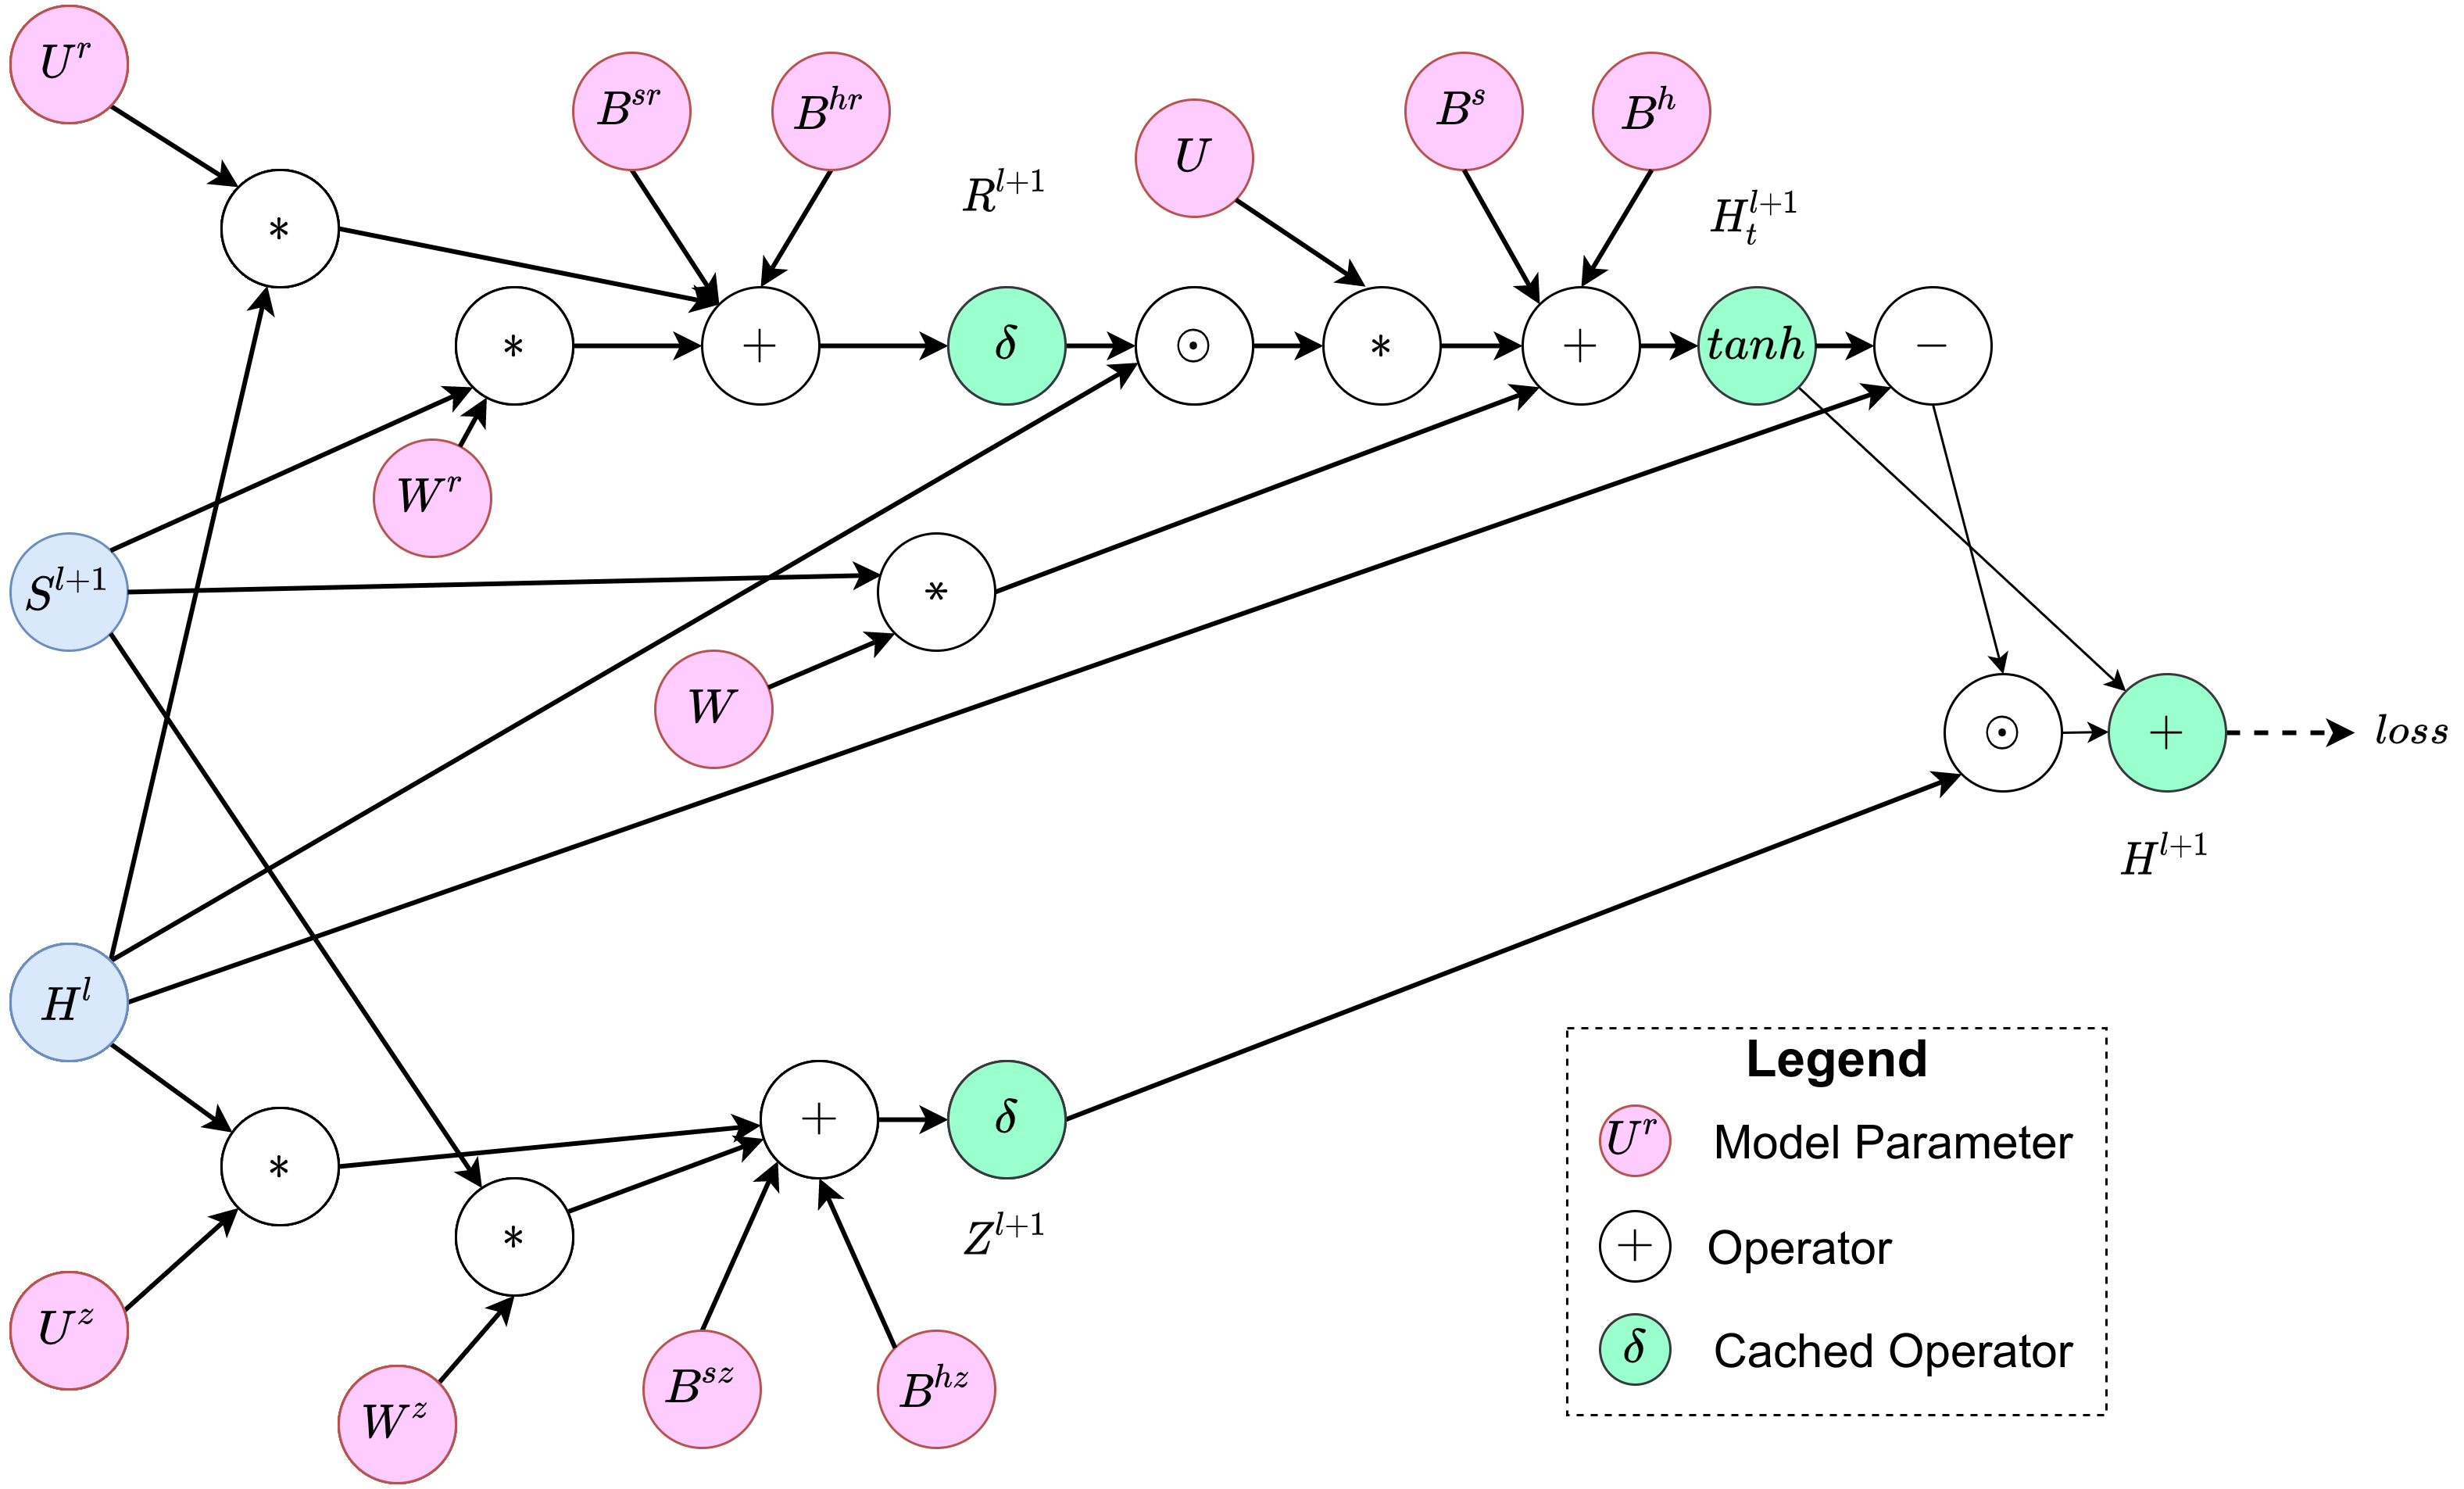
\includegraphics[width=0.7\columnwidth]{figs/illustration/ggnn_vertex_func_computation_graph.png}
    \caption{The calculation graph of the GGNN vertex calculation function $\gamma$. The output of the Cached Operator will be cached for gradient calculation in the backward process}
    \label{fig:ggnn_vertex_func_computation_graph}
\end{figure}

It is worth noting that \textbf{the peak memory during GNN training far exceeds the memory usage of the dataset itself}.
The ratio of the highest peak memory usage during our training compared to the memory usage after data Load is
defined as the memory expansion ratio. \figurename~\ref{fig:exp_memory_expansion_ratio} compares the memory expansion ratios
of different GNNs on different datasets. The expansion ratio of GCN is the lowest, between 5-14 times,
and the expansion ratio of GaAN is the highest, up to 101 times.
\textbf{Very high expansion ratio severely limits the data scalability of GNN, making GPU unable to process large-scale graph datasets},
especially restricting GNN with high edge calculation complexity.

\begin{figure}
    \centering
    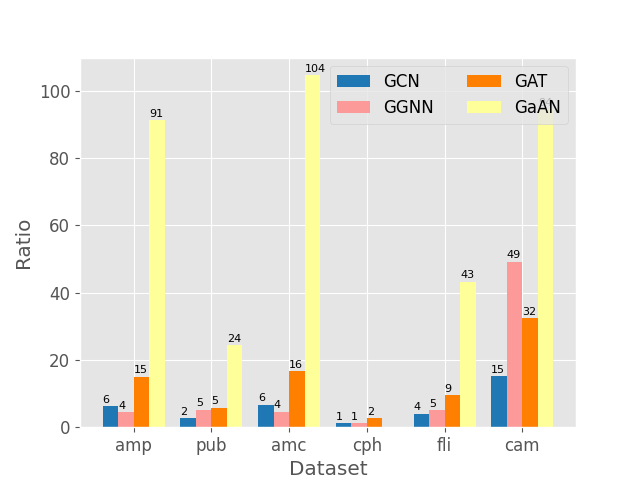
\includegraphics[width=0.7\columnwidth]{figs/experiments/exp_memory_expansion_ratio.png}
    \caption{The proportion of memory expansion of each GNN on different datasets.}
    \label{fig:exp_memory_expansion_ratio}
\end{figure}

\figurename~\ref{fig:exp_memory_expansion_ratio} also shows that the expansion ratio of the same GNN under the same hyperparameters changes with different datasets.
Because the input feature dimension of the \textit{cph} dataset is much higher than the hidden vector of the GNN layer The dimension of the input feature vector matrix
of the graph is much higher than the matrix size of the intermediate calculation result of the cache,
so its expansion ratio is particularly low, and the cam dataset is the opposite. In order to measure the effect of the input feature vector dimension on the memory
expansion ratio , We randomly generated feature vectors of specific dimensions for different datasets.
\figurename~\ref{fig:exp_memory_expension_ratio_input_feature_dimension} shows the change in the expansion ratio under different input feature vector dimensions.
\textbf{In the same GNN structure and hyperparameter settings, using a higher-dimensional input feature vector can reduce memory expansion ratio} .

\begin{figure}
    \centering
    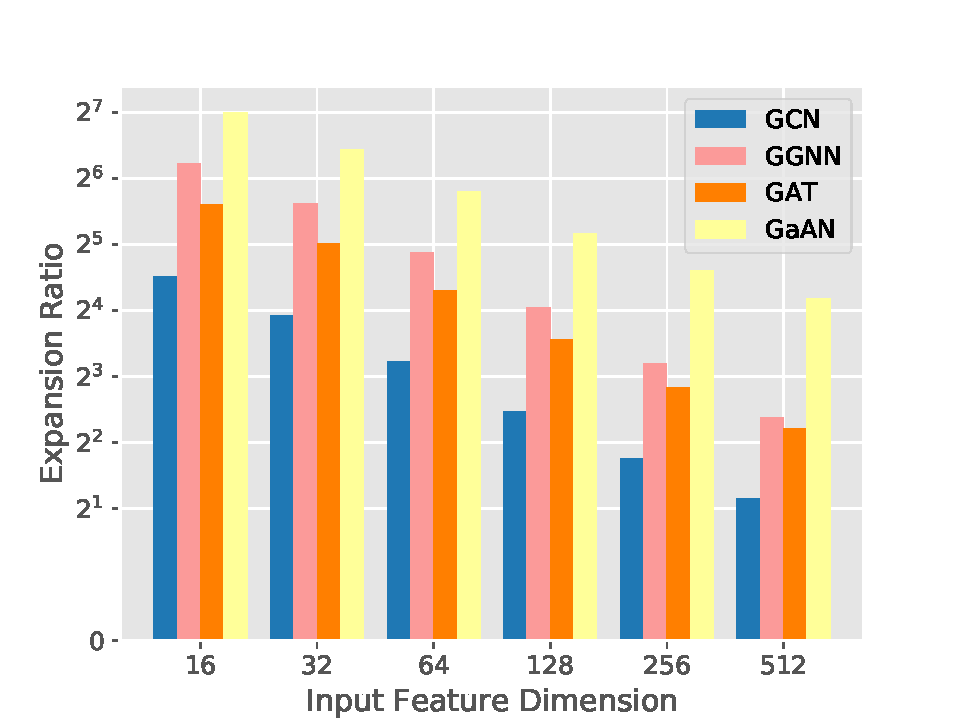
\includegraphics[width=0.7\columnwidth]{figs/experiments/exp_memory_expansion_ratio_input_feature_dimension_com-amazon.pdf}
    \caption{The change of the memory expansion ratio with the dimension of the input feature vector. dataset: cam, other datasets are similar}
    \label{fig:exp_memory_expension_ratio_input_feature_dimension}
\end{figure}

Different GNNs have different vertex/edge calculation complexity, and the scale of the generated intermediate results has different sensitivity
to the number of vertices/edges in the graph, resulting in the memory expansion ratio being affected by the average degree of the graph.
We measured the GPU peak memory The usage and expansion ratios are affected by the scale of the graph.

In the case of a fixed number of vertices in the graph, we use the R-MAT generator to generate random graphs with different average degrees (number of edges).
The \figurename~\ref{fig:exp_memory_expansion_ratio_input_graph_number_of_edges} shows how the memory usage during training varies with the average degree.
\textbf{As the average degree increases, the peak memory usage increases linearly.
    The intermediate results generated by the edge calculation gradually dominate, and the memory expansion ratio of each GNN gradually stabilizes}.
The expansion ratio is affected by the complexity of the edge calculation.
Except for GGNN, the memory expansion ratio of other GNNs increases with the increase of degree. GGNN has a high vertex calculation complexity.
When the average degree is low, its memory expansion ratio is mainly affected by the intermediate results of vertex calculation;
when the average When the degree is increased, the memory expansion ratio is gradually determined by the edge calculation complexity.
Because GGNN has the lowest edge calculation complexity, its stable expansion ratio is the lowest.

\begin{figure}
    \centering
    \subfloat[]{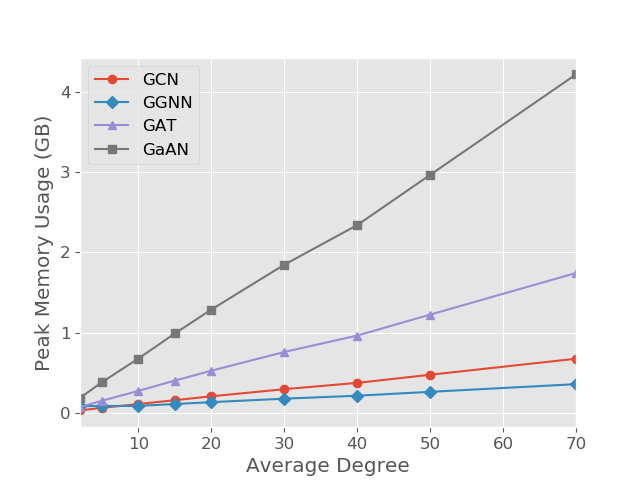
\includegraphics[height=4cm]{figs/experiments/exp_memory_expansion_ratio_input_graph_number_of_edges_peak_memory.png}}
    \subfloat[]{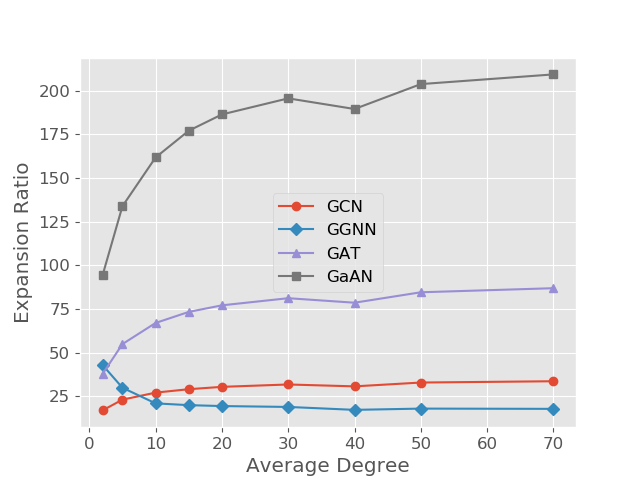
\includegraphics[height=4cm]{figs/experiments/exp_memory_expansion_ratio_input_graph_number_of_edges_expansion_ratio.png}}
    \caption{The change of memory usage with the average degree of the graph (R-MAT random graph, the number of vertices is fixed at 10k, and the input feature vector dimension is 32}
    \label{fig:exp_memory_expansion_ratio_input_graph_number_of_edges}
\end{figure}

In the case of a fixed number of edges in the graph, we use the R-MAT generator to generate random graphs with different numbers of vertices
\figurename~\ref{@fig:exp_memory_expansion_ratio_input_graph_number_of_vertices_fixed_edge} shows the change of memory usage with the number of vertices during training.
Except for GGNN, the number of vertices increases, the number of vertices increases, the number of vertices increases,
and the number of vertices increases. The size of the eigenvector matrix of the vertex input becomes larger,
but the peak memory usage only increases slightly, which makes the proportion of memory expansion decrease to a certain extent.
Only GGNN has a large number of intermediate calculation results during the vertex calculation process because of the high vertex calculation complexity.
The memory expansion factor has a small increase. The experimental data shows that \textbf{the intermediate result produced by the edge calculation is the dominant factor
    in memory usage, and the peak memory usage of each GNN increases linearly with the increase in the number of edges}.

\begin{figure}
    \centering
    \subfloat[]{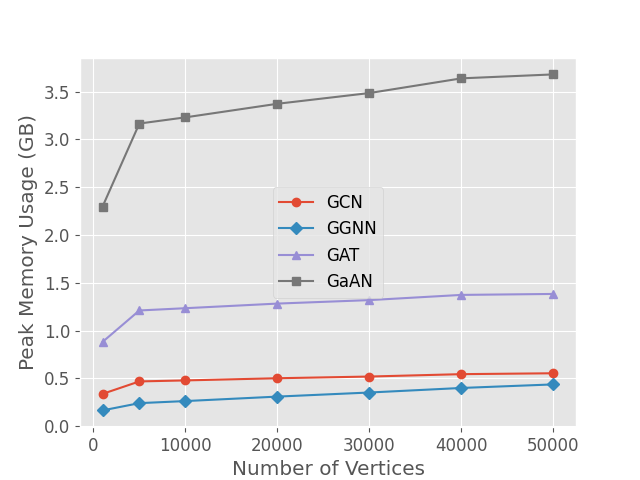
\includegraphics[height=4cm]{figs/experiments/exp_memory_expansion_ratio_input_graph_number_of_vertices_fixed_edge_peak_memory.png}}
    \subfloat[]{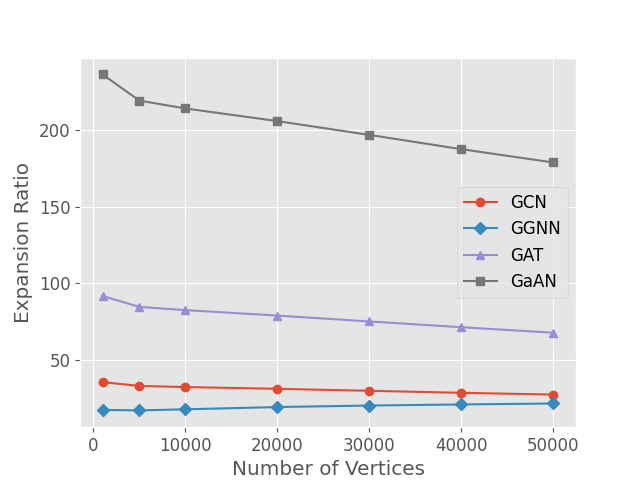
\includegraphics[height=4cm]{figs/experiments/exp_memory_expansion_ratio_input_graph_number_of_vertices_fixed_edge_expansion_ratio.png}}
    \caption{Memory usage changes with the number of graph vertices (R-MAT random graph, the number of edges is fixed at 500k, and the input feature vector dimension is 32)}
    \label{fig:exp_memory_expansion_ratio_input_graph_number_of_vertices_fixed_edge}
\end{figure}

\paragraph{Bottleneck restricting data scalability}
\begin{itemize}
    \item \textbf{GPU memory capacity is the decisive factor limiting the scalability of the training dataset}.
    \item \textbf{GPU memory usage mainly comes from the intermediate calculation results generated during the calculation process,
              especially the intermediate calculation results of the edge calculation. Because part of the intermediate calculation results
              will be cached to participate in backward calculation, high GPU memory usage runs through the forward and backward stages.}
    \item \textbf{GNN's peak memory usage during training can reach tens or even hundreds of times the size of the input data. The limited memory capacity of the GPU severely limits the size of the input data that can be trained}.
    \item \textbf{In the case of a fixed number of vertices, The peak memory usage of GNN increases linearly with the increase of the number of edges of the graph, The proportion of memory expansion will gradually stabilize to a fixed value determined by the complexity of the edge calculation}.
    \item \textbf{In the case where the network structure and various hyperparameters are fixed, using a higher-dimensional input feature vector can reduce the expansion ratio of GPU memory usage}.
\end{itemize}

\label{sec:memory_usage_analysis}
\subsection{Effects of Sampling Techniques on Performance}

Before the sampling technique, GNN training is full batch, that is, all the vertices and edges in the training set participate in the training and calculate the gradient at the same time.
Full batch training can ensure convergence, but the training overhead is large each time, resulting in slow convergence.
Inspired by the minibatch training method in stochastic gradient descent, a series of GNN sampling techniques are proposed.
The sampling technique decomposes the training of the full graph (i.e. epoch) into several batches, and
each batch uses only part of the graph vertices and edges to participate training and performing gradient
updates greatly reduces the training time of each batch, allowing multiple rounds of gradient descent to
be performed within a fixed time, thereby accelerating convergence. The experiments in this section mainly
analyze the impact of sampling techniques on training performance.

In the current implementation of PyG, the GNN model parameters always reside on the GPU,
and the dataset resides in the main memory. When processing each epoch, the CPU samples
the graph dataset in the main memory and generates several batches,
Each batch is a small-scale subgraph of the dataset. When training each batch,
PyG copies the subgraph data corresponding to the batch to the GPU's memory,
trains based on the subgraph and updates the model parameters according to the gradient.
Based on the sampling technology and SGD optimization technology,
the evaluation of the model parameters is performed every several epochs.
The evaluation can be carried out on the CPU or on the GPU.
Therefore, the statistical data in the experiments in this section does not include the evaluation phase.
Neighbor Sampler and Cluster Sampler is selected in this section as they are two typical graph sampling techniques for analysis.

\figurename~\ref{fig:exp_sampling_minibatch_graph_info} shows how the size of the subgraph sampled in the two sampling techniques varies with the batch size.
For Neighbor Sampler, the relative batch size is equal to the number of vertices sampled in the last layer of GNN relative to the top of the full graph the proportion of vertices.
For Cluster Sampler, the batch size is equal to the number of partitions sampled compared to the number of all partitions in the whole graph.
\textbf{Neighbor Sampler is very sensitive to the increase in batch size. As the batch size increases,
    the sampling subgraph The number of vertices/edges and the average degree both increase rapidly and tend to stabilize}.
\textbf{Cluster Sampler is less sensitive to the increase in batch size, the number of vertices/average degree increases
    linearly with the increase in batch size, and the number of edges is in the batch When the size is relatively small,
    it also increases linearly.}

It is worth noting that \textbf{the average degree of the subgraph sampled is much lower than the average degree of the whole graph,
    especially when the relative batch size is low}. Taking Neighbor Sampler at a relative batch size of 6\% as an example,
The average degree of the \textit{amp} dataset is 31.1, but the average degree of the sampled subgraph is only 5.8,
which is much lower than the average degree of the full graph.
The average degree of the subgraph sampled by the Cluster Sampler is lower, only 3.0.
\figurename~\ref{fig:exp_sampling_minibatch_degrees_distribution} shows the comparison of the distribution of the sampled subgraph with the original graph.
The vertex dregree distribution of subgraphs sampled by the two sampling techniques is lower than that of the original graph.
The reason is that the degree distribution of vertex in the actual graph dataset follows a power-rate distribution and only a small number of vertices is very high,
which improves the average degree. In the sampling process, because the sampling method will limit the neighborhood size of the vertex, thereby reducing the upper limit of the vertex degree,
so that the average degree drops significantly. Combined with the experimental results in section 4.2, the decrease in the average degree of sampled subgraph will increase the time-consuming
proportion of vertex calculation. For GGNN with high vertex calculation complexity, vertex calculation will replace edge calculation and become a performance bottleneck.

\begin{figure}
    \centering
    \subfloat[Neighbor Sampler]{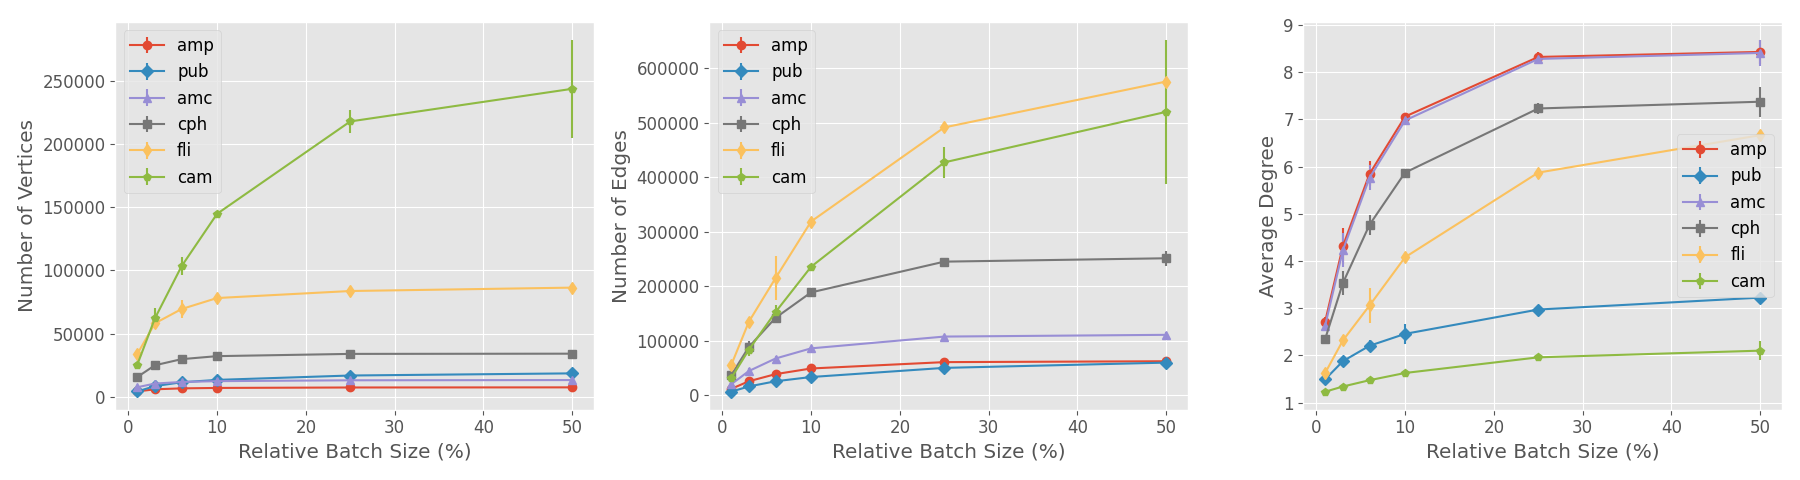
\includegraphics[height=4cm]{figs/experiments/exp_sampling_minibatch_realtive_graph_info_graphsage_gcn.png}} \\
    \subfloat[Cluster Sampler]{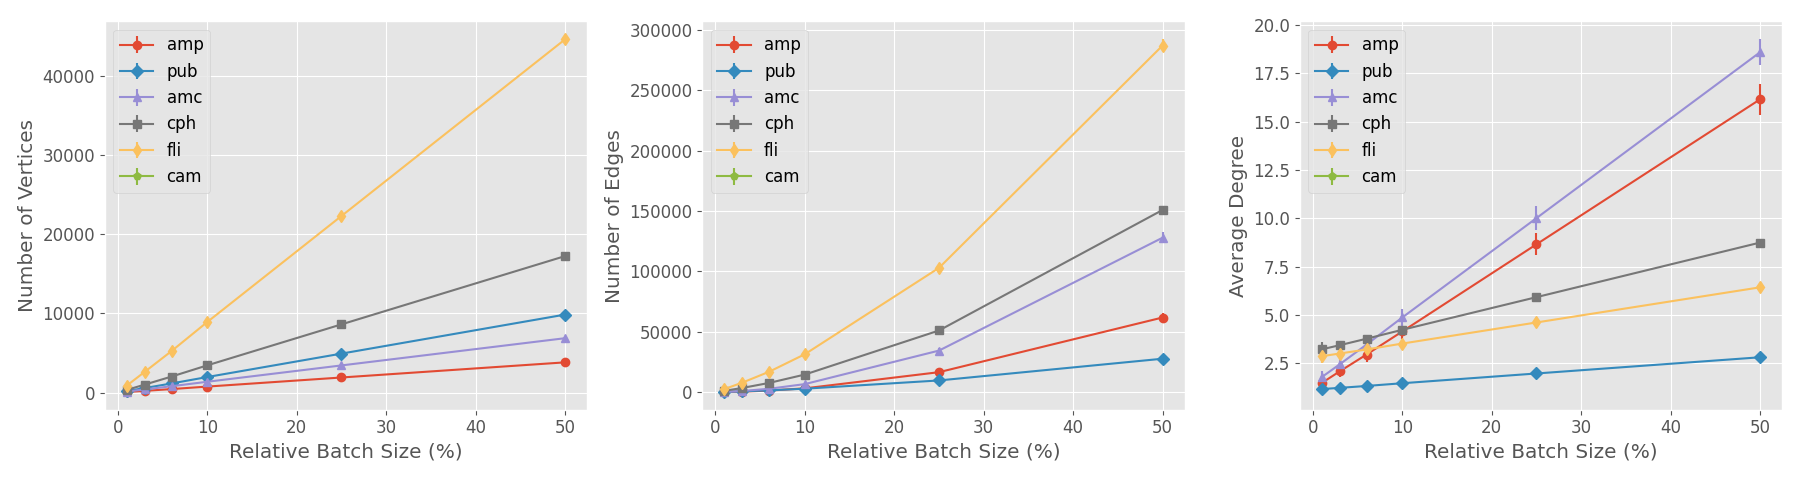
\includegraphics[height=4cm]{figs/experiments/exp_sampling_minibatch_realtive_graph_info_cluster_gcn.png}}
    \caption{The size of the sampled subgraph changes with the batch size. Each batch size is sampled 50 times, and the error bar represents the standard deviation. The relative batch size is the ratio relative to the full graph.)}
    \label{fig:exp_sampling_minibatch_graph_info}
\end{figure}


\begin{figure}
    \centering
    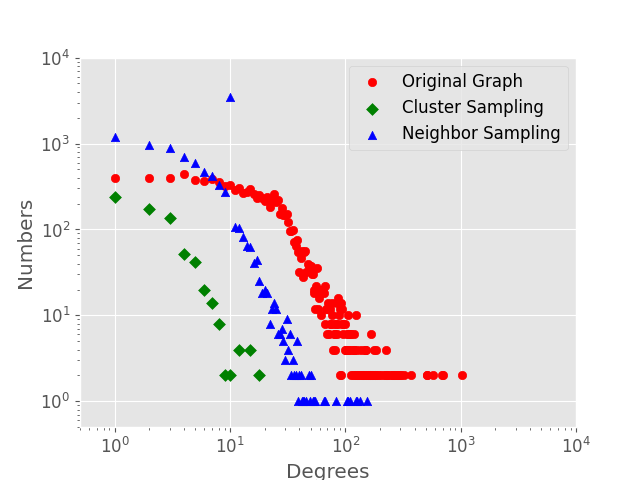
\includegraphics[width=0.7\columnwidth]{figs/experiments/exp_sampling_minibatch_degrees_distribution_amazon-photo.png}
    \caption{Comparison of the vertex degree distribution of the sampled subgraph and the original graph. dataset: amp. Batch size = 512 (Neighbor Sampler) / 20 (Cluster Sampler)}
    \label{fig:exp_sampling_minibatch_degrees_distribution}
\end{figure}

\figurename~\ref{fig:exp_sampling_batch_train_time} shows the change of the training time of each batch on the \textit{amc} and \textit{fli} datasets with the batch size after using the sampling technique.
For the Neighbor Sampler, the time spent in the training phase is significantly reduced compared to full-batch training only when the batch size is very small.
When the batch size is particularly small, the training time is significantly reduced. However, because the sampling itself has additional overhead,
and there is also an overhead in transferring the sampled subgraph to the GPU, the training time of the entire batch may exceed the full graph.
training is time-consuming. For Cluster Sampler, the sampled subgraph is smaller than Neighbor Sampler under the same relative batch size,
which makes the effect of sampling technology more obvious. But when the relative batch size increases,
the increment by additional cost of sampling technology is very obvious. When the relative batch size $\geq$ 25\%,
the total time of each batch of the sampling technique even exceeds the time of the full graph training.
Experiments show that \textbf{the implementation of sampling technology in PyG at this stage is very inefficient and the extra overhead is high}.
When the batch size is slightly larger, the additional cost of sampling technology accounts for more than 50\% of the total training cost of the entire batch.
\textbf{Sampling technology can reduce training time only on very small batches}.

\begin{figure}
    \centering
    \subfloat[Neighbor Sampler on amc]{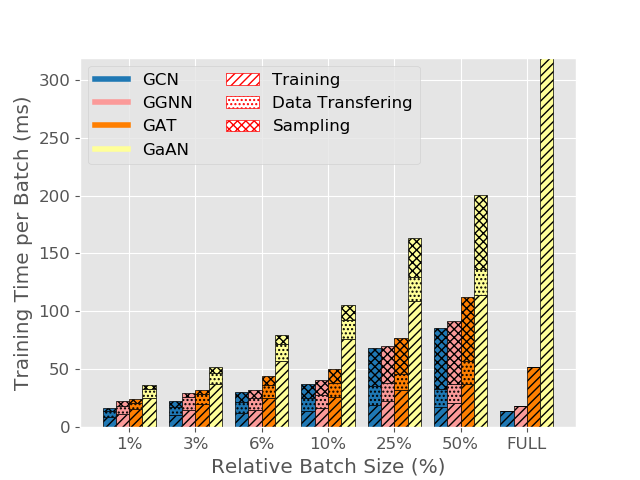
\includegraphics[height=4cm]{figs/experiments/exp_sampling_relative_batch_size_train_time_stack_graphsage_amazon-computers.png}}
    \subfloat[Neighbor Sampler on fli]{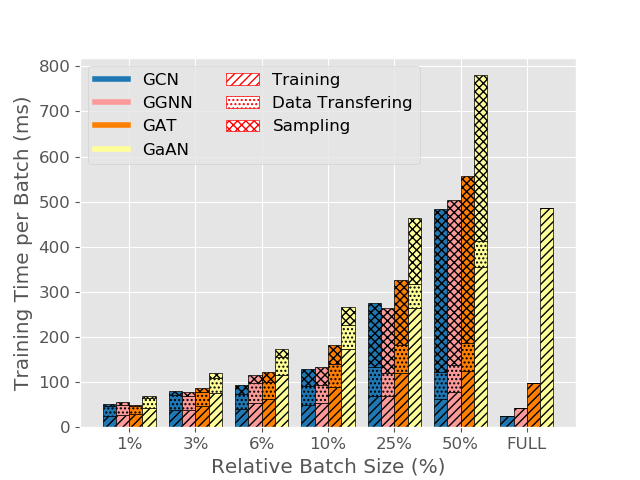
\includegraphics[height=4cm]{figs/experiments/exp_sampling_relative_batch_size_train_time_stack_graphsage_flickr.png}} \\
    \subfloat[Cluster Sampler on amc]{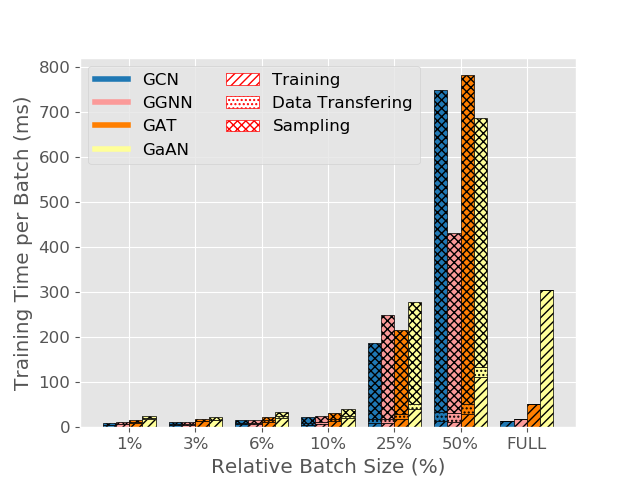
\includegraphics[height=4cm]{figs/experiments/exp_sampling_relative_batch_size_train_time_stack_cluster_amazon-computers.png}}
    \subfloat[Cluster Sampler on fli]{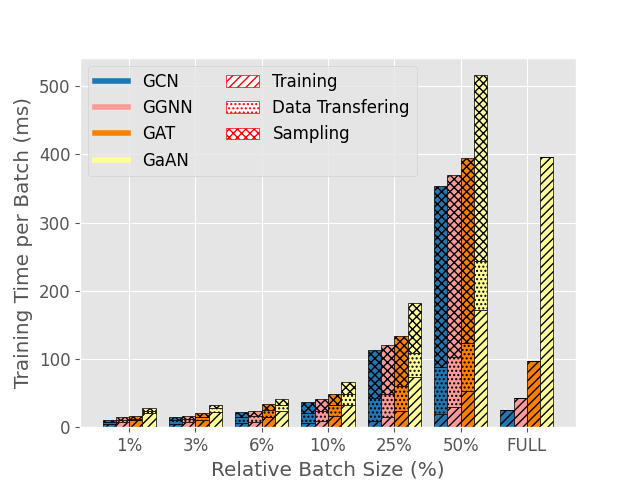
\includegraphics[height=4cm]{figs/experiments/exp_sampling_relative_batch_size_train_time_stack_cluster_flickr.png}}
    \caption{The training time of each batch changes with the batch size. FULL means that the full graph participates in the training phase (excluding evaluation).}
    \label{fig:exp_sampling_batch_train_time}
\end{figure}

However, \textbf{the advantage of the sampling technique is that it can greatly reduce the peak memory usage overhead,
    making large-scale graph neural network training possible}.
\figurename~\ref{fig:exp_sampling_memory_usage} shows how the peak memory usage changes with the relative batch size during the training process after sampling technology is used.
After sampling sampling technology, peak memory usage is greatly reduced and the decrease of Cluster Sampler is greater than that of Neighbor Sampler.

\begin{figure}
    \centering
    \subfloat[Neighbor Sampler on amc]{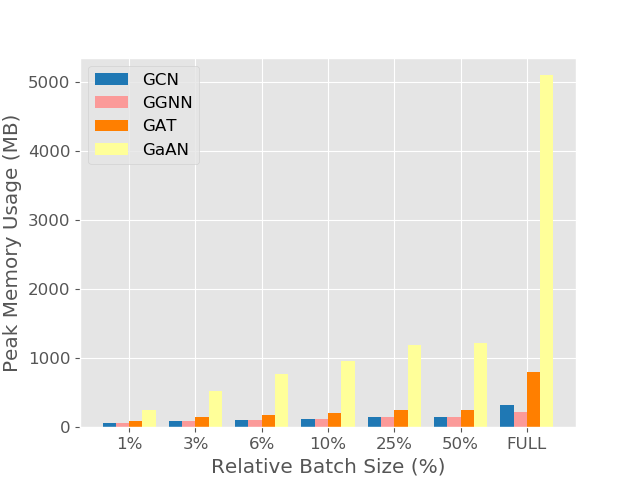
\includegraphics[height=4cm]{figs/experiments/exp_sampling_memory_usage_relative_batch_size_graphsage_amazon-computers_peak_memory.png}}
    \subfloat[Neighbor Sampler on fli]{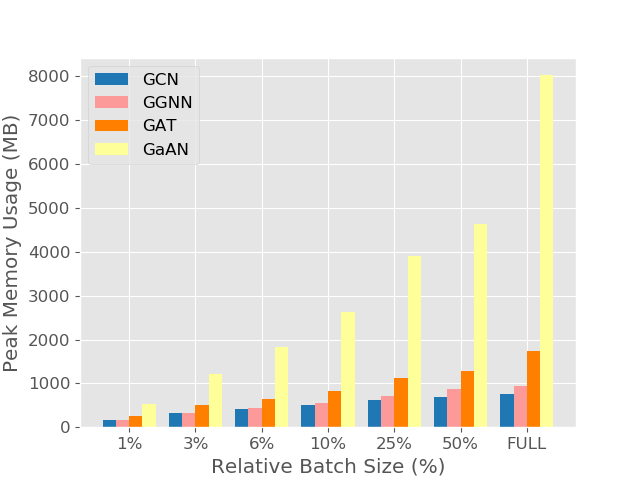
\includegraphics[height=4cm]{figs/experiments/exp_sampling_memory_usage_relative_batch_size_graphsage_flickr_peak_memory.png}} \\
    \subfloat[Cluster Sampler on amc]{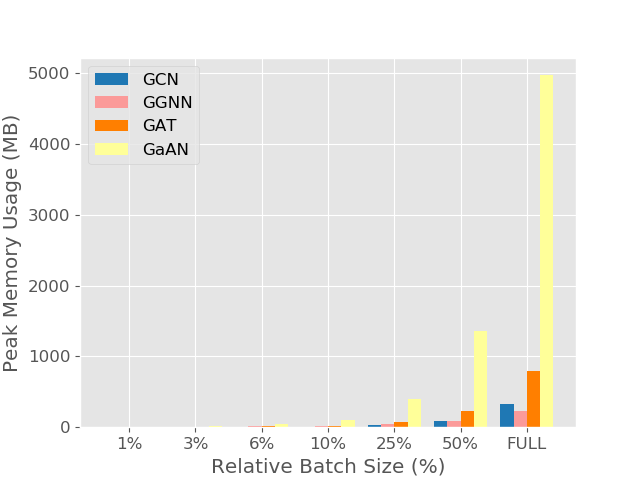
\includegraphics[height=4cm]{figs/experiments/exp_sampling_memory_usage_relative_batch_size_cluster_amazon-computers_peak_memory.png}}
    \subfloat[Cluster Sampler on fli]{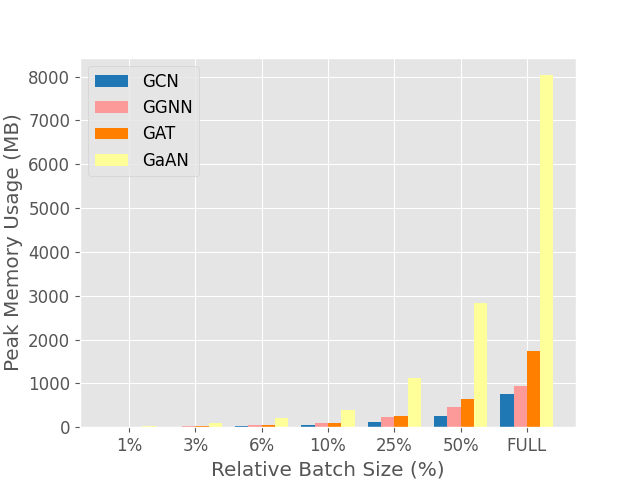
\includegraphics[height=4cm]{figs/experiments/exp_sampling_memory_usage_relative_batch_size_cluster_flickr_peak_memory.png}}
    \caption{Change in peak memory usage with batch size. FULL indicates the case when the sampling technique is not used (excluding the evaluation stage).}
    \label{fig:exp_sampling_memory_usage}
\end{figure}
\label{sec:effects_of_sampling_techniques_on_performance}
